\PassOptionsToPackage{table}{xcolor}
\documentclass[whitelogo]{latex/tudelft-report}
%\documentclass[whitelogo]{tudelft-report}
\usepackage{natbib}
\usepackage{changes}

% Allow Euro sign in .uml file attachments.
\UseRawInputEncoding

% Compile cover
\usepackage{pdfpages}

\usepackage{cleveref}

%rotated image
\usepackage{lscape}
\usepackage{rotating}
\usepackage{pdflscape}

\usepackage{url} %To be able to use url in references

\usepackage{cleveref} %cleverref needs to stand below amsmath package.
\usepackage{appendix}
\crefname{appsec}{Appendix}{Appendices} % refer to appendix as appendix iso as section

% floating figures
\usepackage{float}

% side by side images
\usepackage{subfig}

% Auto scale images
\makeatletter
\newbox\image@box%
\newdimen\image@width%
\newdimen\image@height%
\newcommand\IncludeGraphics[2][\@empty]{%
  \setbox\image@box=\hbox{\includegraphics[#1]{#2}}%
  %\setbox\image@box=\vbox{\includegraphics[#1]{#2}}%
  \image@width\wd\image@box%
  \image@height\ht\image@box%
  \ifdim \image@width>\linewidth%
    \setbox\image@box=\hbox{\includegraphics[width=\linewidth]{#2}}%
    \box\image@box%
  \else
    \ifdim \image@height>0.8\textheight%
       \setbox\image@box=\vbox{\includegraphics[height=0.8\textheight]{#2}}%
     \box\image@box%    
     \else%
       \includegraphics[#1]{#2}%
     \fi%
  \fi%
}


\usepackage[utf8]{inputenc}
% Include glossary list and acrynym list (and include it in the toc)
%\usepackage[acronym,automake,nomain,nonumberlist,toc]{glossaries}
%%%\usepackage[acronym,nomain,nonumberlist,toc]{glossaries}
\usepackage[acronym,toc]{glossaries}
\usepackage[intoc]{nomencl}
\makenomenclature
\makeglossaries

%% Green checkmarks
\usepackage{xcolor,pifont}
\newcommand*\colourcheck[1]{%
  \expandafter\newcommand\csname #1check\endcsname{\textcolor{#1}{\ding{52}}}%
}
%% Red Cross
\newcommand*\colourmark[1]{%
  \expandafter\newcommand\csname #1mark\endcsname{\textcolor{#1}{\ding{55}}}%
}
%% Black Cross
\newcommand{\xmark}{\ding{55}}%


\colourcheck{blue}
\colourcheck{green}
\colourcheck{orange}
\colourcheck{red}

%% Coloured alternating table rows
%\usepackage[table]{xcolor}    % loads also »colortbl«

%%%%%%%%%%%%%%%%%%%%%%%%%%%%%%%%%%%%%%%% End Create listings (Matlab)  %%%%%%%%%%%%%%%%%%%%%%%%%%%%%%%%%%%%%%%%


%%%%%%%%%%%%%%%%%%%%%%%%%%%%%%%%%%%%%%%% Start Create listings (Python)  %%%%%%%%%%%%%%%%%%%%%%%%%%%%%%%%%%%%%%%%
%%%%%%%%%%%%%%%%%%%%%%%%%%%%%%%%%%%%%%%%%%%%%%%%%% Create listings (Python)
% set code color pattern (for python)
% Default fixed font does not support bold face
\DeclareFixedFont{\ttb}{T1}{txtt}{bx}{n}{12} % for bold
\DeclareFixedFont{\ttm}{T1}{txtt}{m}{n}{12}  % for normal

% Custom colors
\usepackage{color}
\definecolor{deepblue}{rgb}{0,0,0.5}
\definecolor{deepred}{rgb}{0.6,0,0}
\definecolor{deepgreen}{rgb}{0,0.5,0}

\usepackage{listings}

% Python style for highlighting
\newcommand\pythonstyle{\lstset{
language=Python,
breaklines=true, % wrap lines
postbreak=\mbox{\textcolor{red}{$\hookrightarrow$}\space}, % wrap lines
basicstyle=\ttm,
otherkeywords={self},             % Add keywords here
keywordstyle=\ttb\color{deepblue},
emph={MyClass,__init__},          % Custom highlighting
emphstyle=\ttb\color{deepred},    % Custom highlighting style
stringstyle=\color{deepgreen},
frame=tb,                         % Any extra options here
showstringspaces=false            % 
}}

% Python environment
\lstnewenvironment{python}[1][]
{
\pythonstyle
\lstset{#1}
}
{}

% Python for external files
\newcommand\pythonexternal[2][]{{
\pythonstyle
\lstinputlisting[#1]{#2}}}

% Python for inline
\newcommand\pythoninline[1]{{\pythonstyle\lstinline!#1!}}
%%%%%%%%%%%%%%%%%%%%%%%%%%%%%%%%%%%%%%%% End Create listings (Python)  %%%%%%%%%%%%%%%%%%%%%%%%%%%%%%%%%%%%%%%%




% Include verbatim txt file
% Source: https://tex.stackexchange.com/questions/85200/include-data-from-a-txt-verbatim
%\usepackage[dvipsnames]{xcolor}
\usepackage{fancyvrb}

% redefine \VerbatimInput
\RecustomVerbatimCommand{\VerbatimInput}{VerbatimInput}%
{fontsize=\footnotesize,
 %
 frame=lines,  % top and bottom rule only
 framesep=2em, % separation between frame and text
 %rulecolor=\xcolor{Gray},
 %
 label=\fbox{\color{Black}data.txt},
 labelposition=topline,
 %
 commandchars=\|\(\), % escape character and argument delimiters for
                      % commands within the verbatim
 commentchar=*        % comment character
}


% Determine whether it is local compilation or overleaf compilation
\makeatletter
\begingroup\endlinechar=-1\relax
       \everyeof{\noexpand}%
       \edef\x{\endgroup\def\noexpand\homepath{%
         \@@input|"kpsewhich --var-value=HOME" }}\x
\makeatother
\def\overleafhome{/tmp}% change as appropriate

% Include boolean to hide source code 
% (requested by financier).
\newif\ifhidesourcecode
%\hidesourcecodetrue % Set the variable value to true.
\hidesourcecodefalse % Set the variable value to false.

\begin{document}



%% Use Roman numerals for the page numbers of the title pages and table of
%% contents.
\frontmatter

%% Uncomment following 19 lines for a cover with a picture on the lower half only
%\title[tudelft-white]{Title}
%\subtitle[tudelft-cyan]{Optional subtitle}
%\author[tudelft-white]{J.\ Random Author}
%\affiliation{Technische Universiteit Delft}
%\coverimage{cover.jpg}
%\titleoffsetx{10cm}
%\titleoffsety{10cm}
%\afiloffsetx{1cm}
%\afiloffsety{18cm}
%\covertext[tudelft-white]{
%    \textbf{Cover Text} \\
%    possibly \\
%    spanning 
%    multiple 
%    lines
%    \vfill
%    ISBN 000-00-0000-000-0
%}
%\makecover

%% Uncomment following 16 lines for a cover with a picture on the lower half only
\title[tudelft-white]{Leveraging brain adaptation to increase radiation resistance of neuromorphic space hardware}

\subtitle[tudelft-black]{\vspace{1em}AE5810 Thesis Project: baseline report}
\author[tudelft-white]{\vspace{2em}Akke Toeter}
\affiliation{Technische Universiteit Delft}
%TODO :include detection of compilation platform
\coverimage{latex/cover1.jpeg}
%\coverimage{cover2.jpg}
%\coverimage{cover3.jpeg}

\covertext[tudelft-white]{
	\vspace{20em}
    \textbf{Supervisors} \\
    TU Delft:\\
    \phantom{text}  Dr. D.M. Stam\\
    \phantom{text} Dr. A. Menicucci\\
    Radboud University: \\
    \phantom{text} Dr. J.H.P. Kwisthout
    \vfill
    %ISBN 000-00-0000-000-0
}
\setpagecolor{tudelft-cyan}
\makecover[split]


%% Include an optional title page.
%TODO :include detection of compilation platform
\begin{titlepage}


\begin{center}

%% Insert the TU Delft logo at the bottom of the page.

%% Print the title in cyan.
{\makeatletter
\largetitlestyle\fontsize{26}{26}\selectfont\@title
%\largetitlestyle\color{tudelft-cyan}\Huge\@title
\makeatother}

%% Print the optional subtitle in black.
{\makeatletter
\ifx\@subtitle\undefined\else
    \bigskip
   {\tudsffamily\fontsize{18}{20}\selectfont\@subtitle}    
    %\titlefont\titleshape\LARGE\@subtitle
\fi
\makeatother}

\bigskip
\bigskip

by
%door

\bigskip
\bigskip

%% Print the name of the author.
{\makeatletter
%\largetitlefont\Large\bfseries\@author
\largetitlestyle\fontsize{16}{26}\selectfont\@author
\makeatother}

\bigskip
\bigskip

Systems Engineering component of the AE5810 Thesis
%ter verkrijging van de graad van Master of Science

at the Delft University of Technology.
%aan de Technische Universiteit Delft,

%in het openbaar de verdedigen op dinsdag 1 januari om 10:00 uur.

\vfill

\begin{tabular}{lll}
    Student number: & 1507958\\
    Project Planning duration: & \multicolumn{2}{l}{September 20, 2020 -- September 24, 2021} \\
    Version: & 0.1 \\
    %Tracking changes w.r.t \textit{previous version}: & Included new chapter 4 - \textit{Knowledge Basis} that investigates\\
        %& the sub-questions defined to sensibly narrow down the\\
        %& research question.
    %Thesis committee: & Prof.\ dr.\ ir.\ J.\ Doe, & TU Delft, supervisor \\
    %    & Dr.\ E.\ L.\ Brown, & TU Delft \\
    %    & Ir.\ A.\ Aaronson, & Acme Corporation
\end{tabular}
%% Only include the following lines if confidentiality is applicable.

\bigskip
\bigskip
%\emph{This thesis is confidential and cannot be made public until December 31, 2013.}
%\emph{Op dit verslag is geheimhouding van toepassing tot en met 31 december 2013.}

\bigskip
\bigskip
%An electronic version of this thesis is available at \url{http://repository.tudelft.nl/}.
%\\[1cm]

%\centering{
\includegraphics{cover/logo_black}}


\end{center}

\begin{tikzpicture}[remember picture, overlay]
    \node at (current page.south)[anchor=south,inner sep=0pt]{
    	%TODO :include detection of compilation platform
        
\includegraphics{latex/project6/cover/logo_black}
    };
\end{tikzpicture}

\end{titlepage}

%\section*{Preface}
\setheader{Preface}

Preface\ldots

\begin{flushright}
{\makeatletter\itshape
    \@author \\
    Delft, January 2013
\makeatother}
\end{flushright}



\tableofcontents

%% Use Arabic numerals for the page numbers of the chapters.
\mainmatter




%\input{chapters/4_summary}

\ifx\homepath\overleafhome
% Overleaf compilation.

% Include acronym list
% Nomenclature is a list of abbreviations and their description.
% Source: https://www.overleaf.com/learn/latex/Glossaries
% All before begin document
%\usepackage[utf8]{inputenc}
%\usepackage[acronym,toc]{glossaries}

\newacronym{alu}{ALU}{Arithmatic Logic Unit}
\newacronym{ann}{ANN}{Artificial Neural Network}
\newacronym{bit}{BIT}{Binary Digit}
\newacronym{biser}{BISER}{Built-in Soft Error Resillience}
\newacronym{bios}{BIOS}{Basic Input/Output System}
\newacronym{bjt}{BJT}{Bipolar Junction Transistor}
\newacronym{cme}{CME}{Coronal Mass Ejection}
\newacronym{cmos}{CMOS}{Complementary Metal–Oxide–Semiconductor}
\newacronym{cpu}{CPU}{Central Processing Unit}
\newacronym{dec}{DEC}{Double-error Correcting Code}
\newacronym{esa}{ESA}{European Space Agency}
\newacronym{dice}{DICE}{Dual Interlocked Storage Cell}
\newacronym{dnn}{DNN}{Deep Neural Network}
\newacronym{dnu}{DNU}{Dual-node Upset}
\newacronym{dod}{DOD}{Department of Defence}
\newacronym{dram}{DRAM}{Dynamic Random Access Memory}
\newacronym{ecc}{ECC}{Error Correction Code}
\newacronym{elt}{ELT}{Enclosed Layout Transistor}
%\newacronym{enc}{ENC}{Effective Nuclear Charge}
%https://en.wikipedia.org/wiki/Effective_nuclear_charge
\newacronym{fet}{FET}{Field-Effect Transistor}
\newacronym{ffd}{FFD}{Functional Flow Diagram}
\newacronym{fbd}{FBD}{Functional Break-down Diagram}
\newacronym{gcd}{GCD}{Greatest Common Divisor}
\newacronym{gcr}{GCR}{Galactic Cosmic Ray}
\newacronym{ic}{IC}{Integrated Circuit}
\newacronym{inrc}{INRC}{Intel Neuromorphic Research Community}
\newacronym{lcm}{LCM}{Least Common Multiple}
\newacronym{let}{LET}{Linear Energy Transfer}
\newacronym{mpnn}{MPNN}{Multilayer Perceptron Neural Network}
\newacronym{mos}{MOS}{Metal–Oxide–Semiconductor}
\newacronym{mosfet}{MOSFET}{Metal–Oxide–Semiconductor Field-Effect Transistor}
\newacronym{msn}{MSN}{Mission Need Statement}
\newacronym{nvm}{NVM}{Non-Volatile Memory}
\newacronym{pos}{POS}{Project Objective Statement}
\newacronym{ram}{RAM}{Random Access Memory}
\newacronym{rdt}{RDT}{Requirements Discovery Tree}
\newacronym{rom}{ROM}{Read Only Memory}
\newacronym{sec}{SEC}{Single-error Correcting Code}
\newacronym{see}{SEE}{Single-event Effects}
\newacronym{seib}{SEIB}{Single-event Induced Burnout}
\newacronym{segr}{SEGR}{Single-event Gate Rupture}
\newacronym{sel}{SEL}{Single-event Latch-up}
\newacronym{ser}{SER}{Soft-error Rate}
\newacronym{serl}{SERL}{Soft-error Resilient Latch}
\newacronym{set}{SET}{Single-event Transient}
\newacronym{seu}{SEU}{Single-event Upset}
\newacronym{ses}{SES}{Single-event Snapback}
\newacronym{snn}{SNN}{Spiking Neural Network}
\newacronym{snu}{SNU}{Single-node Upset}
\newacronym{sram}{SRAM}{Static Random Access Memory}
\newacronym{spe}{SPE}{Solar Particle Events}
\newacronym{heynderickx_new_2004}{SPENVIS}{Space Environment Information System}
\newacronym{stdp}{STDP}{Spike-Timing-Dependent Plasticity}
\newacronym{tlb}{TLB}{Translation Lookaside Buffer}% TODO: add to glossary
\newacronym{tmr}{TMR}{Tripple-mode Redundancy}
\newacronym{vlsi}{VLSI}{Very-Large-Scale Integration}
\newacronym{wfd}{WFD}{Work Flow Diagram}
\newacronym{wbs}{WBS}{Work Break-down Structure}
%\newacronym{}{}{}
%\printglossary
% Glossary is a list of terms and their description.
% Source: https://www.overleaf.com/learn/latex/Glossaries
% All before begin document
%\usepackage[toc]{glossaries} % if no accronyms are used.
%\usepackage[acronym,toc]{glossaries} at acronyms.tex is sufficient.
%\makeglossaries
%\mbox{}
\newglossaryentry{latex}
{
        name=latex,
        description={Is a mark up language specially suited for 
scientific documents}
}

\newglossaryentry{maths}
{
        name=mathematics,
        description={Mathematics is what mathematicians do}
}

\newglossaryentry{formula}
{
        name=formula,
        description={A mathematical expression}
}

\newglossaryentry{ptypesemiconductor}
{
        name=p-type semiconductor,
        description={A semiconductor that is doped with electron acceptors}
}

\newglossaryentry{ntypesemiconductor}
{
        name=n-type semiconductor,
        description={A semiconductor that is doped with electron donors}
}

\newglossaryentry{pnjunction}
{
        name=p-n junction,
        description={A boundary interface of two  a p-type semiconductor and a n-type semiconductor}
}

\newglossaryentry{holes}
{
        name=(electron) holes,
        description={In the context of doped semiconductors, holes are positions where electron acceptors are located, in other words, they are holes at which the electron can go.}
}

\newglossaryentry{unipolar-transistors}
{
        name=unipolar transistors,
        description={Unipolar transistors are transistors that use either electrons or electron holes as charge carriers and not the combination of the two.}
}
\newglossaryentry{cpu_cache}
{
        name=CPU cache,
        description={A small hardware memory unit that is faster than the main memory and closer to the \acrlong{alu}.}
}
\newglossaryentry{instruction_cache}
{
        name=instruction cache,
        description={A cache that is designed to increase the speed with which instructions are fetched.}
}
\newglossaryentry{data_cache}
{
        name=data cache,
        description={A cache that is designed to increase the speed with which data is fetched and stored.}
}
\newglossaryentry{random-access}
{
        name=random-access,
        description={A memory type that has access times that are independent of its physical location.}
}
\newglossaryentry{memory_cell}
{
        name=memory cell,
        description={A fundamental/basic unit in computing that is used to store information.}
}

\newglossaryentry{primary_memory}
{
        name=primary memory,
        description={A form of memory that is only accessible to the \acrlong{cpu} which reads instructions from it and executes those instructions.}
}

\newglossaryentry{prompt_charge}
{
        name=prompt charge,
        description={The charge that is collected by means of funnelling.} % TODO: verify whether this lose interpretation of:
        %A large fraction of the total charge collected by the circuit node occurs in time periods of about 200 ps, and this is referred to as prompt charge. There is also a delayed component that is collected by diffusion. The delayed component can extend to 1 µs or longer,[2] and is important for slower SEE phenomena such as upset in dynamic memories, and latchup.
        % of:
        %https://radhome.gsfc.nasa.gov/radhome/papers/seeca4.htm
        % is accurate.
}
%\printglossary
% Nomenclature is a list of mathematical symbols and their description.
% Source: https://www.overleaf.com/learn/latex/Nomenclatures
%\usepackage[intoc]{nomencl}
%\makenomenclature

% Within document
\mbox{}

\nomenclature{$c$}{Speed of light in a vacuum inertial frame}
\nomenclature{$h$}{Planck constant}

% Include chapters.
\chapter{Introduction}\label{chap:baseline_introduction}
This document presents the baseline for the AE5810 Thesis Project of the Space Flight Master at the Faculty of Aerospace Engineering of Delft University of Technology and the SOW-MKI92 Research Project of the Master in Artificial Intelligence at the faculty of Social Sciences of Radboud University. Its purpose is to identify the 2-5 most feasible design options that can be used to determine whether the principle of brain adaptation can be leveraged in neuromorphic space hardware.


The baseline report presents the \acrfull{ffd} and \acrfull{fbd} in \cref{chap:baseline_ffd} and \cref{chap:baseline_fbd} respectively. These function descriptions of the system that is to be designed, is then used to generate the \acrfull{rdt} in \cref{chap:baseline_requirements_discovery_tree}. Next, the resource allocation and budget breakdown presented in \cref{chap:baseline_resource_allocation_budget_breakdown}. This is followed by the technical risk assessment in \cref{chap:baseline_technical_risk_assessment}. From the \acrshort{rdt}, the \acrfull{dot} is generated in \cref{chap:baseline_requirements_discovery_tree}. Contingency management is applied in \cref{chap:baseline_contingency_management}. A market analysis is presented in \cref{chap:baseline_market_analysis}, and the sustainable development strategy is presented in \cref{chap:baseline_sustainable_development_management}. To ensure this work is performed with sufficient quality, the reporting and quality control is presented in \cref{chap:baseline_reporting_and_quality_control}. The baseline is concluded in \cref{chap:baseline_conclusion}.
\chapter{Functional Flow Diagram}\label{chap:baseline_ffd}
To gain insight in the system that is to be designed, a \acrlong{ffd} is generated. This \acrshort{ffd} presents the high level functions that the system should be able to perform, in chronological order. These functions are presented in the flow diagram of \cref{fig:basline_ffd}. 

\begin{figure}[H]
    \centering
    %\includegraphics[width=0.6\linewidth]{Images/Diagrams/trivial_gantt.png}
    \includegraphics[width=0.6\linewidth]{latex/Images/Diagrams/trivial_gantt.png}
    \caption{A functional flow diagram with the high-level functions of the system that is to be designed.}
    \label{fig:baseline_ffd}
\end{figure}

\begin{enumerate}
    \item Initialise \& start space-related function on neuromorphic architecture without brain adaptation implementation.
    \item Initialise \& start space-related function on neuromorphic architecture with brain adaptation implementation.
    \item Endure modelled space radiation on neuromorphic architecture.
    \item Measure space-related function performance without brain adaptation implementation.
    \item Measure space-related function performance with brain adaptation implementation.
    \item Report any performance difference between with- and without brain adaptation.
    \item Determine significance of difference.
\end{enumerate}

From these high level functions, a more detailed functional breakdown diagram is generated.

\section{Detailed Functional Flow Diagram}\label{sec:baseline_detailed_ffd}
\begin{enumerate}
    \item Initialise \& start space-related function on neuromorphic architecture without brain adaptation implementation.    
    \begin{enumerate}
        \item Boot/initialise neuromorphic architecture
        \item Load function.
        \item Load function data.
    \end{enumerate}
    \item Initialise \& start space-related function on neuromorphic architecture with brain adaptation implementation.
    \begin{enumerate}
        \item Boot/initialise neuromorphic architecture
        \item Load brain adaptation.
        \item Load space-related function.
        \item Load space-related function data.
    \end{enumerate}
    \item Render and endure modelled space radiation on neuromorphic architecture.
    \begin{enumerate}
        \item Determine simulated space radiation pattern of neuromorphic space architecture.
        \item Expose neuromorphic architecture to simulated space radiation pattern.
        \item Complete space-related function.
        \item Return results of space-related performance.
    \end{enumerate}
    \item Measure space-related function performance without brain adaptation implementation.
    \begin{enumerate}
        \item Retrieve space-related function output.
        \item Convert space-related function output to score.
    \end{enumerate}
    \item Measure space-related function performance with brain adaptation implementation.
    \item \begin{enumerate}
        \item Retrieve space-related function output.
        \item Convert space-related function output to score.
    \end{enumerate}
    \item Report difference between the scores of the architectures with- and without brain adaptation.
    \item Determine significance of difference.
\end{enumerate}

\subsection{Description}\label{subsec:description}
\begin{enumerate}
    \item Initialise \& start space-related function on neuromorphic architecture without brain adaptation implementation.
    \begin{itemize}
        \item To run a function on the neuromorphic architecture, it will have to be booted and initialised. The function that will be ran on the neuromorphic architecture is space related, to increase the level of representativeness of this study, in terms of space applications. The initalisation allows for loading the space related function that is to be executed. Additionally, the space related function may require (training) data on which it is ran. For example, a Martian rover that has a function that identifies rocks in its environment, may be partially simulated by loading a (labelled) dataset of Martian images.

        To run the function without brain adaptation implementation, allows for the creation of a baseline to which the brain adaptation performance can be compared.
    \end{itemize}
    \item Initialise \& start space-related function on neuromorphic architecture with brain adaptation implementation.
    \begin{itemize}
        \item The intialisation of the brain adaptation implementation can occur, before, during or after the loading of the space related function. Which of these options is selected depends on the more detailed design process.
    \end{itemize}
    \item Endure modelled space radiation on neuromorphic architecture.
    \begin{itemize}
        \item The radiation robustness of the neuromorphic architecture can be tested by exposing the neuromorphic architecture to the radiation that it would experience in a space application. To determine what this radiation is, a relevant space mission and space function are selected. The time, position and orientation of the spacecraft in such a mission is then used to derive the radiation pattern to which the radiation may be exposed. This radiation is pattern is then used to determine to which (simulated) radiation the neuromorphic architecture will be exposed.
    \end{itemize}
    \item Measure space-related function performance without brain adaptation implementation.
    \begin{itemize}
        \item The performance of the space related function without brain adaptation implementaiton on the neuromorphic architecture is measured before, during and/or after radiation exposure. Which of these measuring moments are used, is still to be determined by the detailed design process. This measurement then serves as a comparison baseline to put the impact of the brain adaptation implementation into context.
    \end{itemize}
    \item Measure space-related function performance with brain adaptation implementation.
    \item \begin{itemize}
        \item Once a baseline for comparison is established, the space related function can be ran again on the neuromorphic hardware, whilst being exposed to radiation. In this second setting, the brain adaptation implementation is used in an attempt to increase the radiation robustness of the neuromorphic architecture. The performance of the space related function is then measured before, during and/or after radiation exposure. Which of these measuring moments are used, is still to be determined by the detailed design process. 
    \end{itemize}
    \item Report any performance difference between with- and without brain adaptation.
    \item \begin{itemize}
        \item If any performance difference is observed between the space related function with- and without brain adaptation implementation, it will be computed and stored.
    \end{itemize}
    \item Determine significance of difference.
    \item \begin{itemize}
        \item An analysis is performed to determine the level of significance  of any observed difference.
    \end{itemize}
\end{enumerate}
\chapter{Functional Breakdown Diagram}\label{chap:baseline_fbd}
This section presents the functional breakdown diagram of the system that is designed in this thesis project. This \acrshort{fbd} is generated using the detailed functional flow diagram of \cref{sec:baseline_detailed_ffd}. The \acrshort{fbd} presents the activities in an hierarchical style.

\begin{enumerate}
    \item Run space-related function on neuromorphic architecture.
    \begin{enumerate}
        \item Initialise neuromorphic architecture.
        \item Optional: Load brain adaptation implementation.
        \item Load space related function.
        \item Load space related function data.
        \item Run space related function.
        \item Complete running space related function.
        \item Retrieve space related function outputs.
        \item Convert space related function outputs to performance score.
        \item Report difference between the scores of the architectures with- and without brain adaptation.
        \item Determine significance of difference.
    \end{enumerate}
    \item Render and endure modelled space radiation on neuromorphic architecture.
    \begin{enumerate}
        \item Generate simulated space radiation pattern of neuromorphic space architecture.
        \item Expose neuromorphic architecture to simulated space radiation pattern.
        \item Optional: model architecture-radiation interaction.
        \item Optional: measure architecture-radiation interaction.
    \end{enumerate}
\end{enumerate}
\chapter{Requirements Discovery Tree}\label{chap:baseline_requirements_discovery_tree}
This section presents an overview of the requirements that are identified within this thesis project. Its purpose consists of listing the requirements that drive the design, identifying killer requirements and presenting an overview of the project requirements. \cref{sec:baseline_mission_need_statement} contains the mission need statement of this project. Next, the stakeholder requirements are identified in \cref{sec:baseline_stakeholder_requirements}. The top level requirements are presented in \cref{sec:baseline_top_level_requirements}, and the key requirements are presented in \cref{sec:baseline_identification_key_requirements}. From these combined requirements, the \acrlong{rdt} is drafted in \cref{sec:baseline_requirements_discovery_tree}.

\section{Mission Need Statement}\label{sec:baseline_mission_need_statement}
The mission need statement is generated in the project plan phase, and is included in this section again to provide the context of the requirement derivation process. The \acrshort{msn} is:

\textit{Increase the radiation robustness of neuromorphic space hardware by leveraging the principle of brain adaptation in neuromorphic hardware.}

\section{Stakeholder Requirements}\label{sec:baseline_stakeholder_requirements}
The following stakeholder requirements are identified:
\begin{itemize}
    \item \textbf{STKH-UNI-01} - The research that is performed shall be reproducible.
    \item \textbf{STKH-UNI-02} - The sustainability of the design concepts shall be taken into account in the design trade-off process.
    \item \textbf{STKH-SPACEBRAINS-01} - Achieve results towards the REACH research by Q2 2022.
    \item \textbf{STKH-SPACEBRAINS-01-a} - Achieve results towards the REACH research by either: 2022-03-01, 2022-04-07, 2022-07-01.
    \item \textbf{STKH-ICONS-01} - Submit paper documenting research results before April 15th, 2022.
    \item \textbf{STKH-ICONS-01-a} - Submit full paper of 6-8 pages, presenting original research, or submit short paper of 3-4 pages that has preliminary results.
    \item \textbf{STKH-ICONS-02} - Upon acceptance for a presentation, submit presentation before July 27th, 2022.
    \item \textbf{STKH-RADBOUD-01} - The research proceedings shall be documented and submitted in a format accepted by Dr. J.H.P. Kwisthout before the SOW-MKI92 Research Project is completed.
    \item \textbf{STKH-RADBOUD-02} - The research for the SOW-MKI92 Research Project shall be performed using at least 28 EC of work.
    \item \textbf{STKH-Delft-01} - The research proceedings shall be documented and submitted in a format accepted by Dr. D.M. Stam and Dr. A. Menicucci before the AE5810 Thesis Project is completed.
    \item \textbf{STKH-Delft-02} - The research for the AE5810 Thesis Project shall be performed using at least 42 EC of work.
\end{itemize}
% Either Q2 2022 implies 3 monts after the last quarterly report, which was February 2022. Or after 3 after January 1st.
% Based on Q3 reports, which were requested on 2021-10-01 (October 2021), Q4 reports would take place on (January 2022). However these Q4 reports were requested at 2022-02-07, implying a delay of 5 weeks.
% Since one more quarter (Q2 2022) is granted to achieve results towards the REACH research, this is supposed to be at (2022-03-01) without delay. With a 5 week delay this would be approximately 2022-04-07. The end of Q2 2022 would be on end of June 2022=start of July=2022-07-01. It is not specified which time is intended.

\section{Top Level Requirements}\label{sec:baseline_top_level_requirements}
The following requirements for this thesis project are identified:
\begin{itemize}
	\item \textbf{TECH-01} - Technology Readiness Level (TRL) of the used technology shall be at least TRL 4 [-].
	\item \textbf{TEST-01} - Radiation robustness shall be tested in terms of algorithmic performance.
	\item \textbf{TEST-02} - The radiation tests shall be technically and economically feasible.
	\item \textbf{TEST-03} - The radiation tests results shall be generated before September 2022.
	\item \textbf{SUS-01} - Sustainability management shall be integrated in each phase of this project.
	\item \textbf{SUS-02} - Sustainability shall be assessed in the design trade-off process.
	\item \textbf{SAF-01} - All participants involved in testing, integrating and operations shall not be exposed to serious danger. %TODO : specify level of danger explicitly.
	\item \textbf{ESA-01} - Throughout this project quarterly reports shall be provided to the SpaceBrains foundation and the \acrfull{esa}.
\end{itemize}

\section{Identification Key Requirements}\label{sec:baseline_identification_key_requirements}
The key requirements are requirements that can render the project infeasible, requirements that drive the design, and/or requirements that induce high risk to project success. Within this thesis project, the following key requirements are identified:
\begin{enumerate}
    \item \textbf{STKH-SPACEBRAINS-01} - Achieve results towards the REACH research by Q2 2022.
    \item \textbf{TECH-01} - Technology Readiness Level (TRL) of the used technology shall be at least TRL 4 [-].
	\item \textbf{TEST-03} - The radiation tests results shall be generated before September 2022.
\end{enumerate}
The \textbf{STKH-SPACEBRAINS-01} requirement significantly drives the design space, as physical radiation tests are not deemed feasible within the given timeframe and project constraints. \textbf{TEST-03} implies a strict time constraint that induces significant risk to project success as it limits the amount of time available for development and scheduling. \textbf{TECH-01} significantly drives the design as it limits the design space to concepts that rely only on technologies of TRL 4 and higher. 

\section{Requirements Discovery Tree}\label{sec:baseline_requirements_discovery_tree}
A requirements' discovery tree is currently omitted due to time constraints.

\chapter{Resource Allocation and Budget Breakdown}\label{chap:baseline_resource_allocation_budget_breakdown}
\chapter{Technical Risk assessment}\label{chap:baseline_technical_risk_assessment}
\chapter{Design Option Structuring Tree}\label{chap:baseline_dot}
The purpose of the design option tree is to find a feasible design option that can satisfy the requirements. This selection process can be an iterative process in case no feasible design option is found in the initial design option tree. By positioning the design options in a tree format, their hierarchical structure becomes visible. The tree is structured such that the most impactful decisions are selected at the top of the tree, whereas more detailed decisions are made at lower levels of the tree. Several subsections are created to  \Cref{fig:baseline_dot} presents the design option tree for this thesis. The nodes in the tree represent design options and child leafs represent design options within a parent design option. For example, a choice may be made to use digital neuromorphic hardware, and within that design space, a particular chip may be selected. Multiple (parallel) design options may be selected. For example, a softwarematic and hardwarematic implementation may be chosen.
\begin{figure}[H]
    \centering
    %\includegraphics[width=0.6\linewidth]{Images/Diagrams/trivial_gantt.png}
    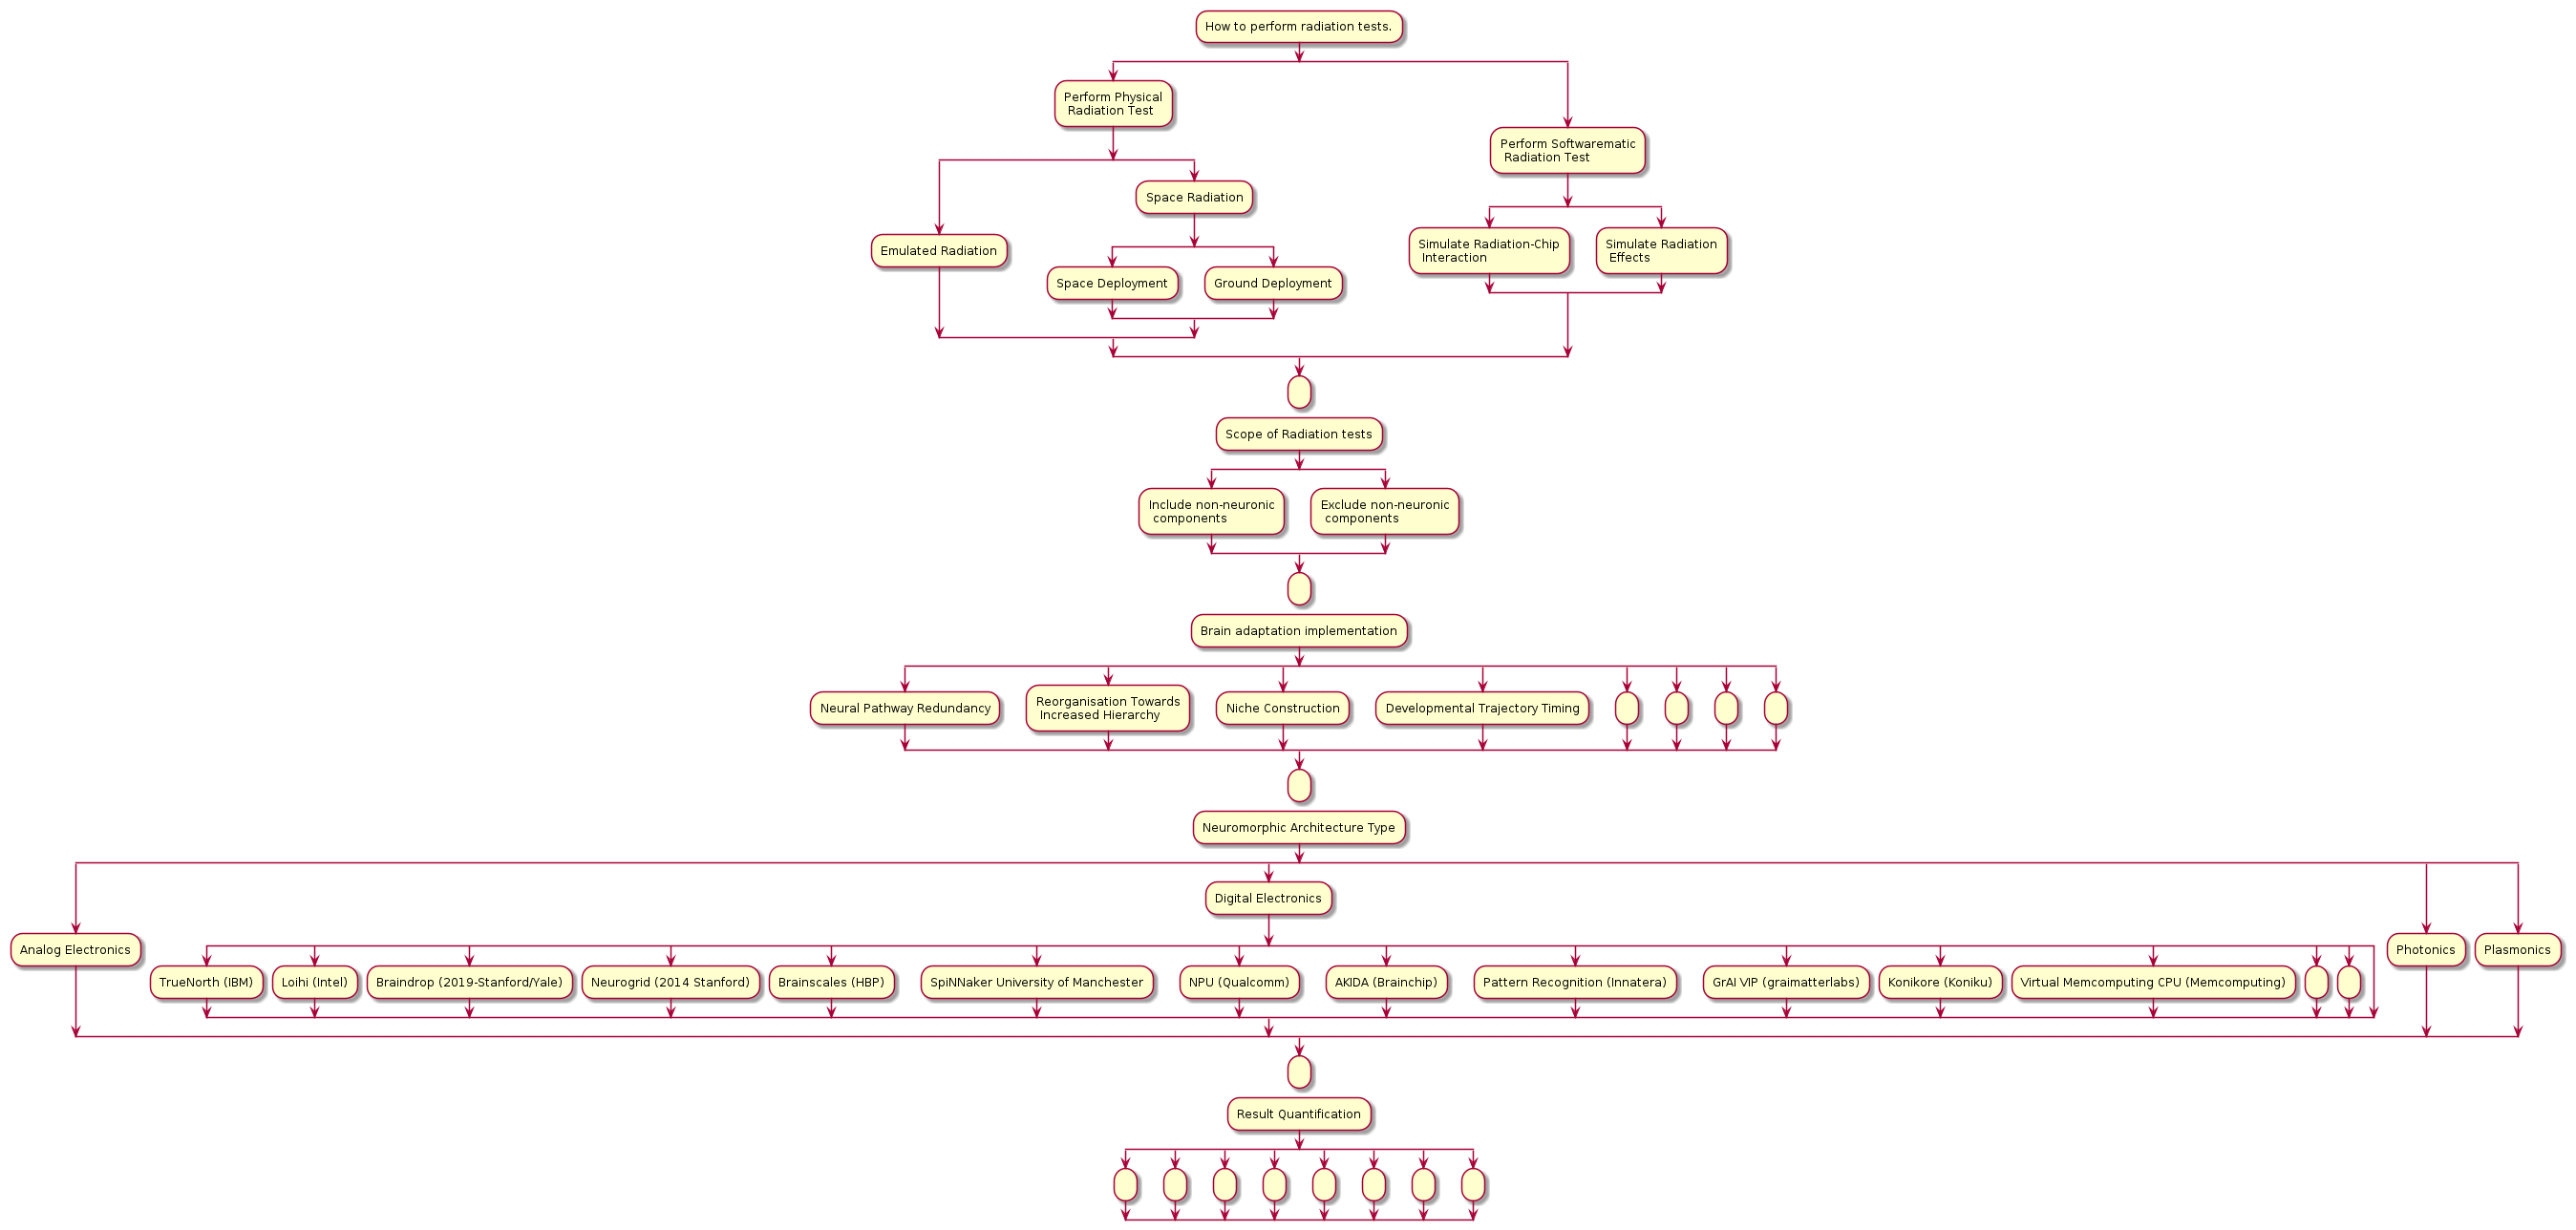
\includegraphics[width=0.6\linewidth]{latex/Images/dot.png}
    \caption{A functional flow diagram with the high-level functions of the system that is to be designed.}
    \label{fig:baseline_dot}
\end{figure}

\section{Pruning}\label{sec:baseline_pruning}
With the design option tree generated, it can be pruned of options that are considered infeasible. This is done using the knowledge base that was generated in the literature study and using the requirements identified in \cref{chap:baseline_requirements_discovery_tree}.  The pruning process will be performed from top to bottom, which matches from high- to low hierarchical design choices.
\subsection{Tested Functionality}\label{subsec:tested_functionality}
At the time of writing, no specific function that is used for testing, can be eliminated.
\subsection{How To Perform Radiation Tests}\label{subsec:baseline_how_to_perform_radiation_tests}
\begin{enumerate}
    \item Starting with key requirement: \textbf{STKH-SPACEBRAINS-01} and \textbf{STKH-ICONS-01}, it is possible to eliminate the physical radiation test design option(along with its children), before the ICONS deadline of April 15th, 2022. Given the full scope of the thesis, and the \textbf{TEST-03} requirement which implies a test deadline before September 2022, a physical radiation test is still considered feasible before that time. Hence, instead of a complete termination (red), it is turned orange.
    \item Continuing with the \textbf{STKH-SPACEBRAINS-01} requirement, it is considered infeasible to do a full simulation of radiation effects on the hardware components, before the ICONS deadline of April 15th, 2022. Hence, also this option will be coloured orange. Most neuromorphic chips in the \acrshort{dot} are proprietary, with many of the chip designs not being publically available. Since that makes it difficult to determine what the radiation effects will be on the hardware components of the chip, and how those effects, such as single-event upsets, would propagate towards influencing neurons and/or synapses. Therefore, this option is not considered feasible before April 15th 2022. It may be possible to contact manufacturers to ask how the radiation influences the neuronal- and synaptic properties. If such research is performed, it may be applied to simulate the neuromorphic hardware-radiation interaction softwarematically with sufficient accuracy to produce meaningful results.
\end{enumerate}   
\subsection{Scope Of Radiation Tests}\label{subsec:baseline_scope_of_radiation_tests}
\begin{enumerate}
    \item For the same as the last enumerated point of \cref{subsec:baseline_how_to_perform_radiation_tests}, including the non-neuromorphic components is not considered feasible for before the ICONS deadline of April 15th, 2022. Hence, this element is also coloured orange.
\end{enumerate}

\subsection{Brain Adaptation Implementation}\label{subsec:baseline_brain_adaptation_implementation}
At the time of writing, no brain adaptation mechanisms can be eliminated.

\subsection{Neuroplasticity Mechanism}\label{subsec:baseline_neuroplasticity_mechanism}
At the time of writing, no neuroplasticitiy mechanisms can be eliminated.

\subsection{Neuromorphic Architecture}\label{subsec:baseline_neuromorphic_architecture}
\begin{enumerate}
    \item Some neuromorphic architectures can be eliminated based on logistical reasons. Currently, the only direct access within this thesis project is to the Loihi. Furthermore, it may be expected that access to Pattern Recognition Chip by Innaterra may be realised after the ICONS deadline. Similarly, the Spinnaker device may become available later-on in the project. An economic feasibility assessment needs to be made on whether they should be used in physical radiation testing or not.
    \item Some of the neuromorphic chip manufacturers have been contacted in the past, these contacts may allow for access to their respective chips for physical radation testing, if the intermediate results at ICONS are promising. Hence, they are kept orange.
\end{enumerate}

\subsection{Result Quantification}\label{subsec:baseline_result_quantification}
\begin{enumerate}
    \item Since physical radiation testing is not deemed possible, and since the hardware diagrams of the respective neuromorphic architectures are not available, it is not deemed feasible to include a radiation effect analysis before ICONS. Therefore, this option is turned orange.
\end{enumerate}

\subsection{Pruned Design Option Tree}\label{subsec:baseline_pruned_dot}
\begin{figure}[H]
    \centering
    %\includegraphics[width=0.6\linewidth]{Images/Diagrams/trivial_gantt.png}
    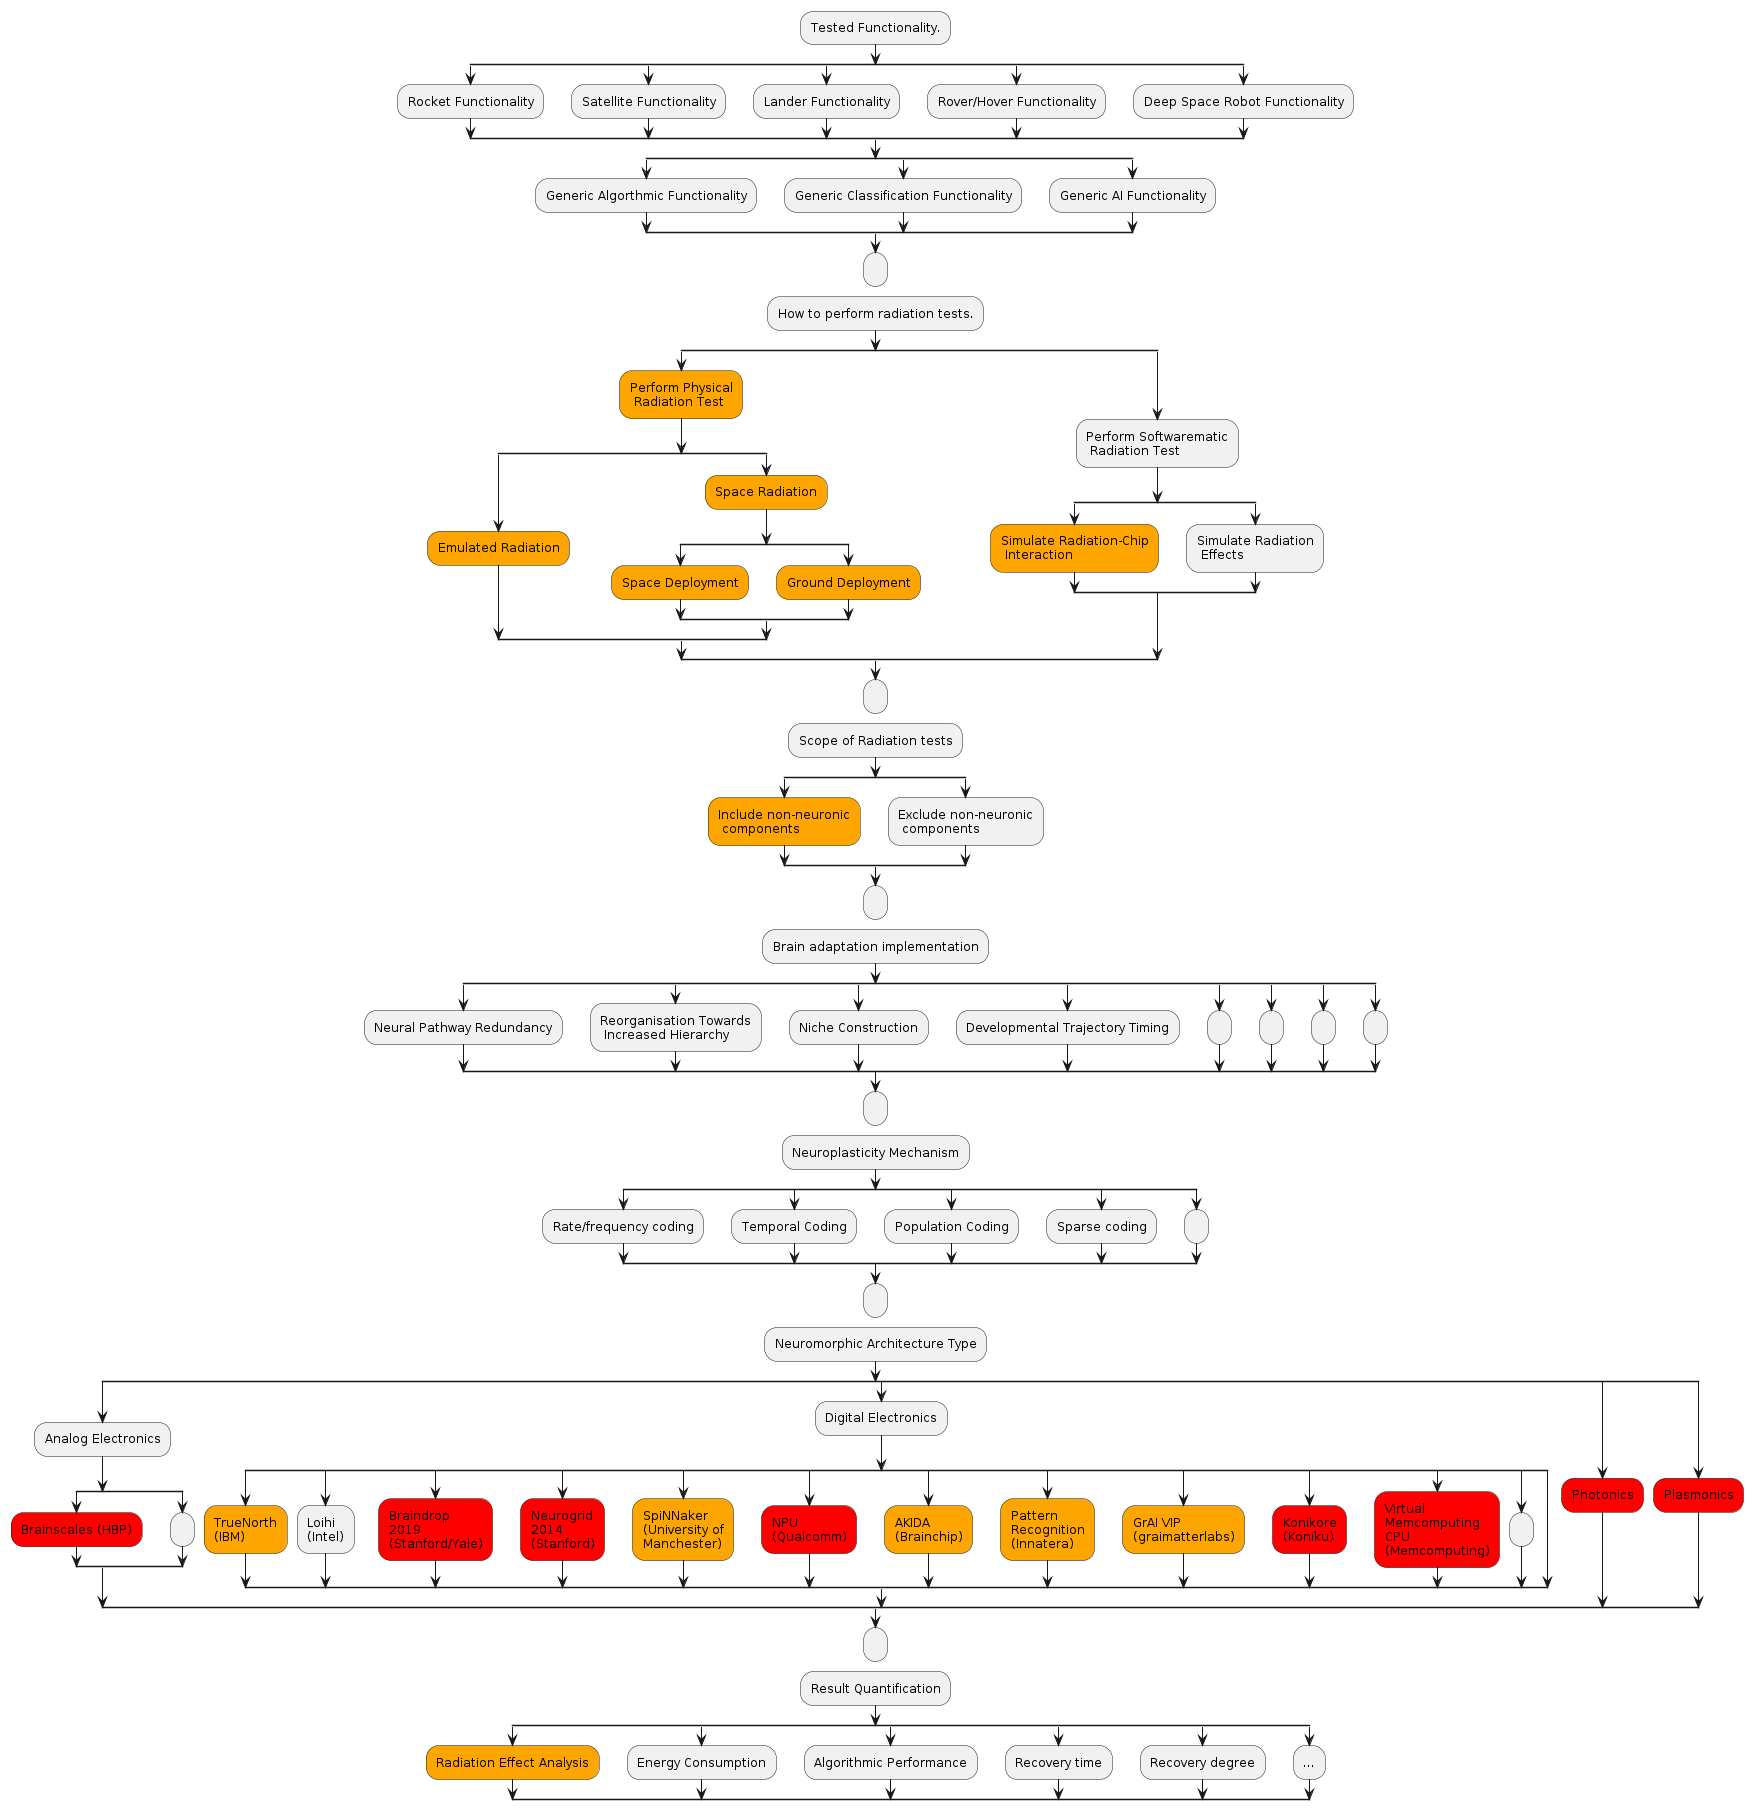
\includegraphics[width=0.6\linewidth]{code/src/Static_diagrams/dot_pruned.png}
    \caption{A functional flow diagram with the high-level functions of the system that is to be designed.}
    \label{fig:baseline_dot}
\end{figure}


\section{Preliminary Design Option Selection}\label{sec:baseline_preliminary_design_option_selection}
With some design options eliminated, an analysis can be performed to see whether some design options are considered to be more feasible than others. This analysis is started by taking the \textbf{STKH-SPACEBRAINS-01} requirement into account, which implies results need to be produced by April 15th. This allows for expressing some design option preferences as listed in \cref{subsec:baseline_tested_functionality_preference} to \cref{subsec:baseline_result_quantification_preference}. Taking the full scope of the thesis project into account allows identification of design options that seem most feasible for a follow-up with physical radiation testing.

\subsection{Tested Functionality Preference}\cref{subsec:baseline_tested_functionality_preference}
For performing a \textit{generic algorithmic functionality} for the following two reasons:
\begin{enumerate}
    \item No additional dependencies such as datasets, panda packages, tensorflow etc. is required. This lowers the probability of allocating time on work that does not directly support the objective of this thesis project.
    \item No preprocessing work, such as loading and/or cropping images etc.,  is required. This increases the amount of time that can be allocated to implementing the brain adaptation and testing its functionality.
    \item Graph algorithms are typically used in space applications \cite{todo}.%, an example is the MDS approximation in communication satellites.
    \item Thorough testing can quickly be set up for graph algorithms.
\end{enumerate}
 
\subsection{How To Perform Radiation Tests Preference}\cref{subsec:baseline_how_to_perform_radiation_tests_preference}
Using softwarematic radiation tests that simulate radiation effects.

\subsection{Scope of Radiation Tests Preference}\cref{subsec:baseline_scope_of_radiation_tests_preference}
Excluding non-neural components from radiation effects allows for a complete focus using the expected radiation effects on the neural and synaptic properties, without having to model additional radiation interactions with (other) hardware elements. This increases the feasibility of producing results by April 15th.

\subsection{Brain Adaptation Implementation Preference}\cref{subsec:baseline_brain_adaptation_implementation_preference}
No preference in brain adaptation implementations is expressed at the time of writing.

\subsection{Neuroplasticity Mechanism Preference}\cref{subsec:baseline_neuroplasticity_mechanism_preference}
No preference in neuroplasticity mechanisms is expressed at the time of writing.

\subsection{Neuromorphic Architecture Type Preference}\cref{subsec:baseline_neuromorphic_architecture_preference}
Based on availability and previous experience, a preference is expressed for the Loihi platform for the softwarematic simulation. Insights from this simulation will be used to determine the best way forward towards hardware simulations. Since the Innatera chips are expected to be available for testing in the second quarter of 2022, combined with there relatively low cost, this option is mentioned as a possible suitable candidate for physical radiation testing. The Spinnaker boards appear to have a higher unit cost.

\subsection{Result Quantification Preference}\cref{subsec:baseline_result_quantification_preference}
Based on the vicinity of the ICONS deadline of April 15th, 2022, a preference is expressed for measuring the softwarematic results in terms of algorithmic performance. This is because it forms the most direct measurement that can be used to determine whether the principle of brain adaptation is indeed able to increase the radiation robustness of neuromorphic space hardware.

\subsection{Preliminary Design Option Tree}\label{subsec:preliminary_design_option_tree}
The preferences expressed in \cref{sec:baseline_preliminary_design_option_selection} are coloured green in the preliminary design option tree visualised in \cref{fig:baseline_preliminary_dot}.

\begin{figure}[H]
    \centering
    %\includegraphics[width=0.6\linewidth]{Images/Diagrams/trivial_gantt.png}
    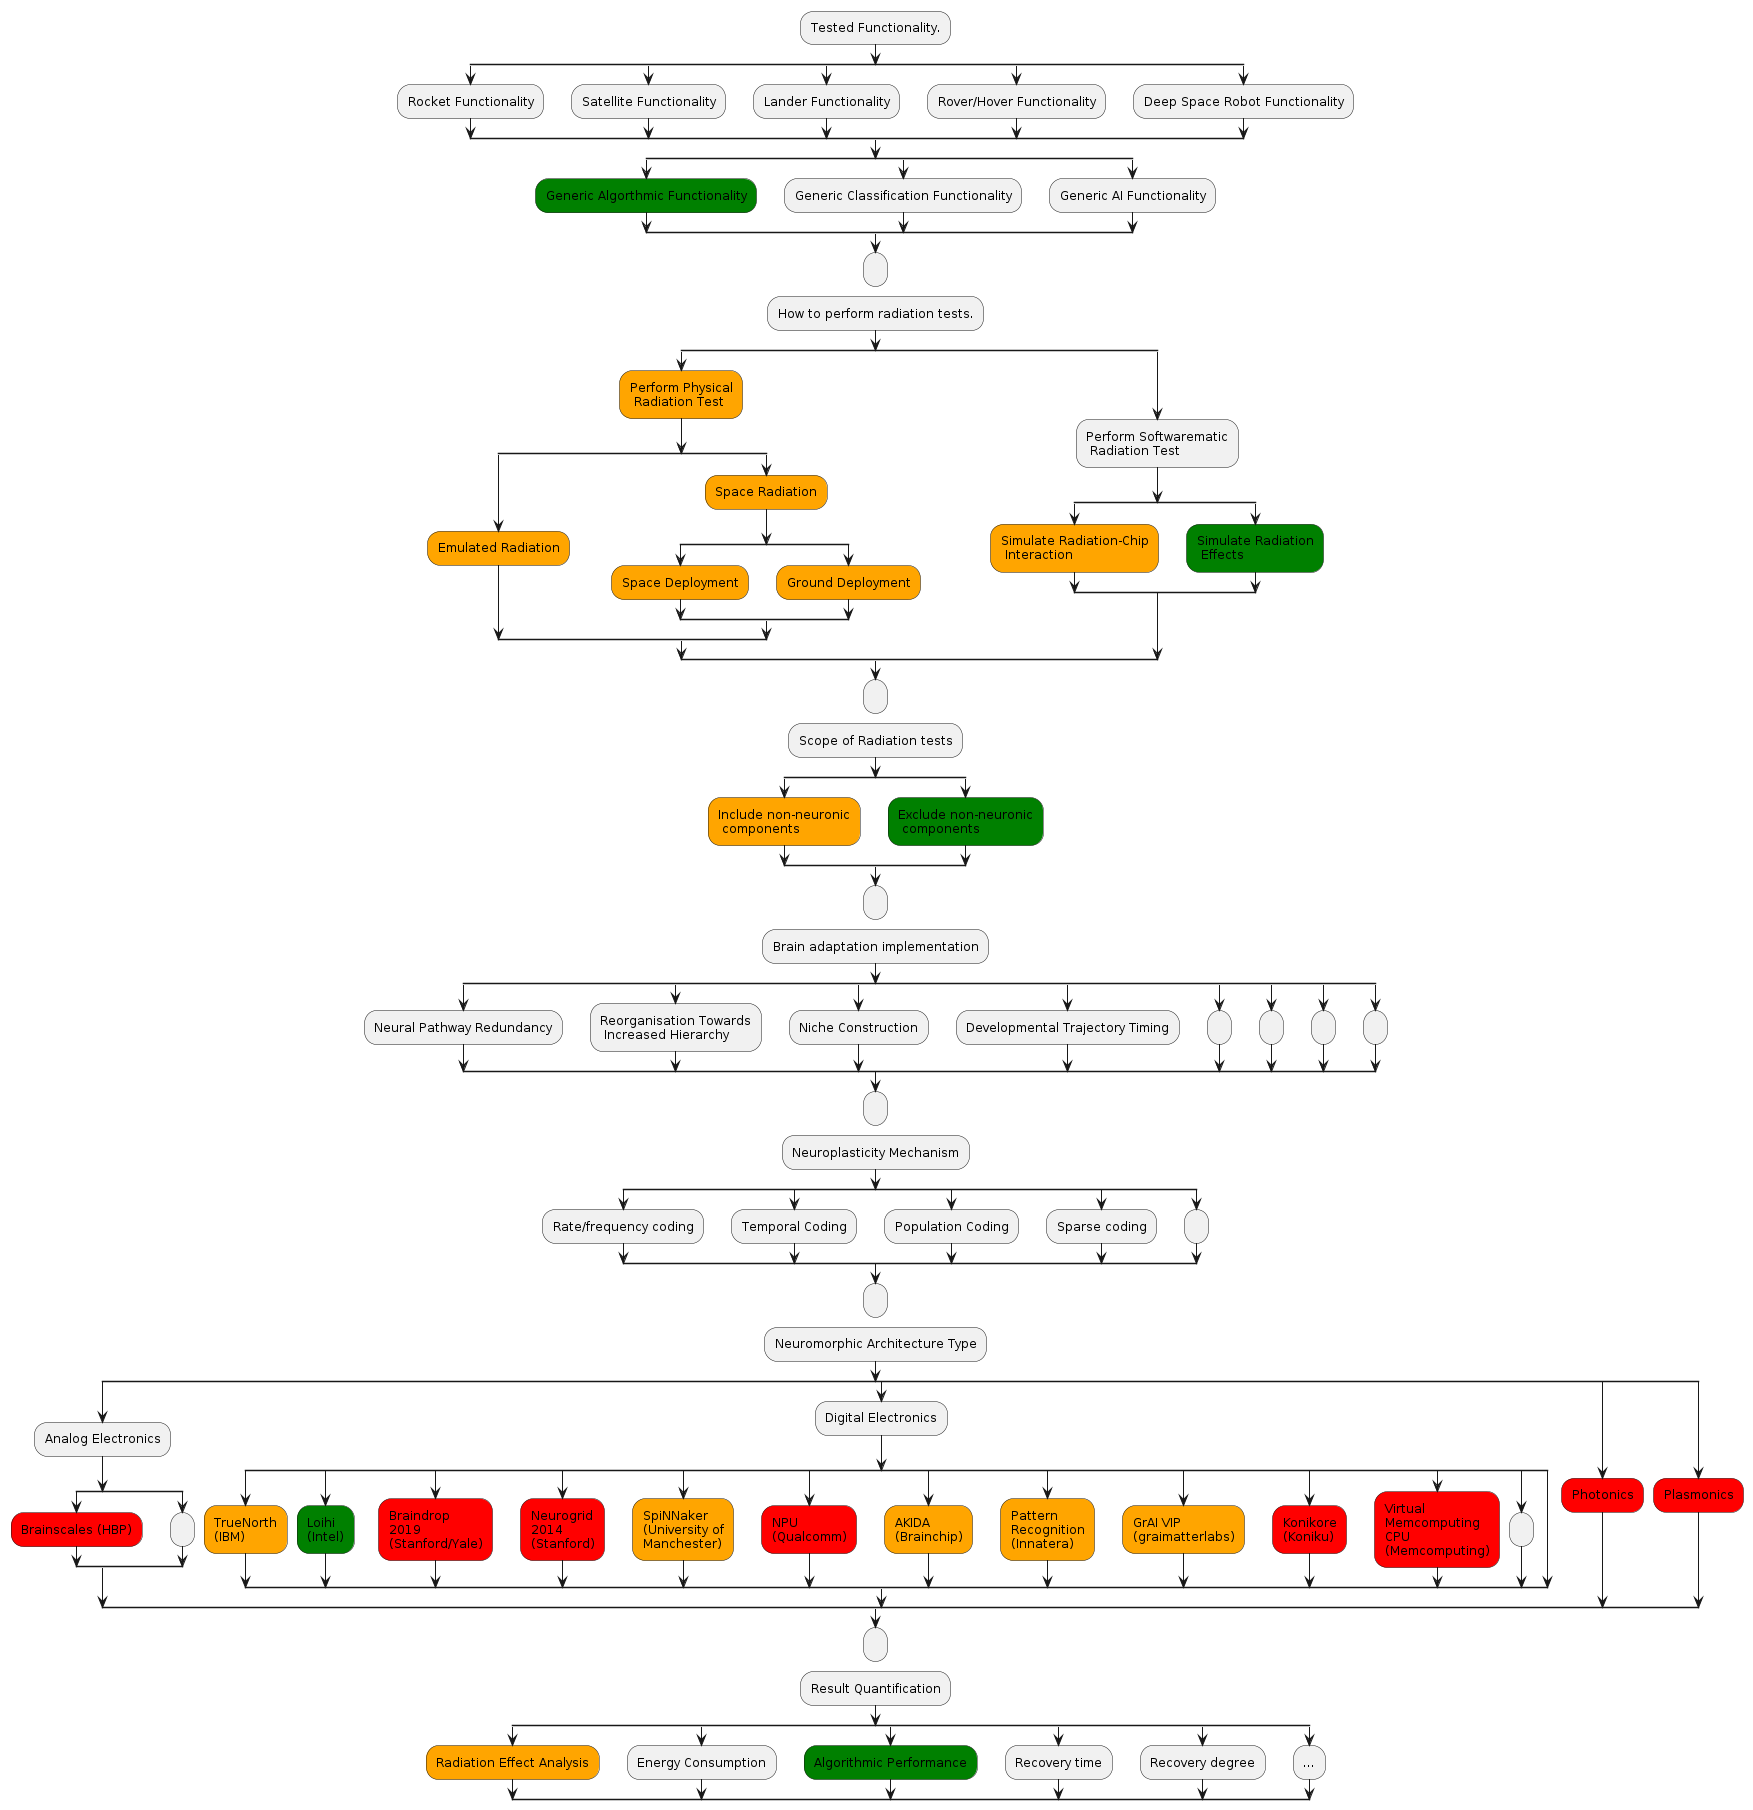
\includegraphics[width=0.6\linewidth]{latex/Images/Diagrams/Static_diagrams/dot_preliminary.png}
    \caption{todo}
    \label{fig:baseline_preliminary_dot}
\end{figure}

\section{Proposed Design options}\label{subsec:baseline_proposed_design options.}
To summarise, a distinction between project phases. First a softwarematic test is performed and the results are reported to the ICONS by  April 15th 2022. Next, a hardwarematic test is proposed that builds upon the knowledge gained in the softwarematic tests. For the first phase, the following options are proposed to be executed during the midterm: A graph algorithm is proposed to be ran, where the radiation effects on the neuromorphic architecture are simulated as changes in the the neural and synaptic properties of the spiking neural networks. For this first softwarematic test, the radiation effects on non-neural/traditional hardware components (such as a memory bus, \acrshort{cpu} etc.) of the neuromorphic architecture are ignored. The Loihi platform will be used for the simulation development and radiation tests. The test results will be interpreted in terms of performance of the graph algorithm. The most feasible brain-adaptation method and neuroplasticitiy mechanism will be determined using hands-on experimentation.
% TODO: change generic alg to graph alg
For the second tests, a physical radiation test is proposed. For this test, the Innatera chips are currently considered as the most feasible option. Based on the results of the softwarematic testing, a decision can be made to inlcude the traditional hardware components of the respective chips. An alternative option could be to apply extra shielding to those components, whilst saving mass on the non-shielded components though the use of brain adaptation inspired implementations.

\chapter{Contingency Management}\label{chap:baseline_contingency_management}
\chapter{Market Analysis}\label{chap:baseline_market_analysis}
\chapter{Sustainable Development Management}\label{chap:baseline_sustainable_development_management}
\chapter{Reporting and Quality Control}\label{chap:baseline_reporting_and_quality_control}
The following quality control compliance checklist can currently be generated for this project plan:

\begin{itemize}
	\item Language Tools Grammar check applied:\greencheck
	\item Language Tools Spelling check applied:\greencheck
	\item CI is ran on code base used in generating this Project Plan:\xmark
	\begin{itemize}
		\item Python Black Formatting Compliance:\xmark
		\item ShellCheck Compliance:\xmark
		\item Latex Prettier Formatting Compliance:\xmark
		\item Python Unit Test Passing: 2 failed, 7 passed [tests]
		\item Python Test Coverage \%:\xmark [\%]
		\item Shell Unit Test Passing:\xmark [tests]
		\item Shell Unit Test Coverage \%:\xmark [\%]
	\end{itemize}
	\item Manual Quality check:
	\begin{enumerate}
		\item Citations still have to be compiled correctly.
		\item Reproduction instructions in Appendix A should be updated.
		\item Word wrap should be applied to .uml appendices.
	\end{enumerate}
\end{itemize}
\chapter{Conclusion}\label{chap:baseline_conclusion}
\else
% Local compilation

% Include acronym list
% Nomenclature is a list of abbreviations and their description.
% Source: https://www.overleaf.com/learn/latex/Glossaries
% All before begin document
%\usepackage[utf8]{inputenc}
%\usepackage[acronym,toc]{glossaries}

\newacronym{alu}{ALU}{Arithmatic Logic Unit}
\newacronym{ann}{ANN}{Artificial Neural Network}
\newacronym{bit}{BIT}{Binary Digit}
\newacronym{biser}{BISER}{Built-in Soft Error Resillience}
\newacronym{bios}{BIOS}{Basic Input/Output System}
\newacronym{bjt}{BJT}{Bipolar Junction Transistor}
\newacronym{cme}{CME}{Coronal Mass Ejection}
\newacronym{cmos}{CMOS}{Complementary Metal–Oxide–Semiconductor}
\newacronym{cpu}{CPU}{Central Processing Unit}
\newacronym{dec}{DEC}{Double-error Correcting Code}
\newacronym{esa}{ESA}{European Space Agency}
\newacronym{dice}{DICE}{Dual Interlocked Storage Cell}
\newacronym{dnn}{DNN}{Deep Neural Network}
\newacronym{dnu}{DNU}{Dual-node Upset}
\newacronym{dod}{DOD}{Department of Defence}
\newacronym{dram}{DRAM}{Dynamic Random Access Memory}
\newacronym{ecc}{ECC}{Error Correction Code}
\newacronym{elt}{ELT}{Enclosed Layout Transistor}
%\newacronym{enc}{ENC}{Effective Nuclear Charge}
%https://en.wikipedia.org/wiki/Effective_nuclear_charge
\newacronym{fet}{FET}{Field-Effect Transistor}
\newacronym{ffd}{FFD}{Functional Flow Diagram}
\newacronym{fbd}{FBD}{Functional Break-down Diagram}
\newacronym{gcd}{GCD}{Greatest Common Divisor}
\newacronym{gcr}{GCR}{Galactic Cosmic Ray}
\newacronym{ic}{IC}{Integrated Circuit}
\newacronym{inrc}{INRC}{Intel Neuromorphic Research Community}
\newacronym{lcm}{LCM}{Least Common Multiple}
\newacronym{let}{LET}{Linear Energy Transfer}
\newacronym{mpnn}{MPNN}{Multilayer Perceptron Neural Network}
\newacronym{mos}{MOS}{Metal–Oxide–Semiconductor}
\newacronym{mosfet}{MOSFET}{Metal–Oxide–Semiconductor Field-Effect Transistor}
\newacronym{msn}{MSN}{Mission Need Statement}
\newacronym{nvm}{NVM}{Non-Volatile Memory}
\newacronym{pos}{POS}{Project Objective Statement}
\newacronym{ram}{RAM}{Random Access Memory}
\newacronym{rdt}{RDT}{Requirements Discovery Tree}
\newacronym{rom}{ROM}{Read Only Memory}
\newacronym{sec}{SEC}{Single-error Correcting Code}
\newacronym{see}{SEE}{Single-event Effects}
\newacronym{seib}{SEIB}{Single-event Induced Burnout}
\newacronym{segr}{SEGR}{Single-event Gate Rupture}
\newacronym{sel}{SEL}{Single-event Latch-up}
\newacronym{ser}{SER}{Soft-error Rate}
\newacronym{serl}{SERL}{Soft-error Resilient Latch}
\newacronym{set}{SET}{Single-event Transient}
\newacronym{seu}{SEU}{Single-event Upset}
\newacronym{ses}{SES}{Single-event Snapback}
\newacronym{snn}{SNN}{Spiking Neural Network}
\newacronym{snu}{SNU}{Single-node Upset}
\newacronym{sram}{SRAM}{Static Random Access Memory}
\newacronym{spe}{SPE}{Solar Particle Events}
\newacronym{heynderickx_new_2004}{SPENVIS}{Space Environment Information System}
\newacronym{stdp}{STDP}{Spike-Timing-Dependent Plasticity}
\newacronym{tlb}{TLB}{Translation Lookaside Buffer}% TODO: add to glossary
\newacronym{tmr}{TMR}{Tripple-mode Redundancy}
\newacronym{vlsi}{VLSI}{Very-Large-Scale Integration}
\newacronym{wfd}{WFD}{Work Flow Diagram}
\newacronym{wbs}{WBS}{Work Break-down Structure}
%\newacronym{}{}{}
%\printglossary
% Glossary is a list of terms and their description.
% Source: https://www.overleaf.com/learn/latex/Glossaries
% All before begin document
%\usepackage[toc]{glossaries} % if no accronyms are used.
%\usepackage[acronym,toc]{glossaries} at acronyms.tex is sufficient.
%\makeglossaries
%\mbox{}
\newglossaryentry{latex}
{
        name=latex,
        description={Is a mark up language specially suited for 
scientific documents}
}

\newglossaryentry{maths}
{
        name=mathematics,
        description={Mathematics is what mathematicians do}
}

\newglossaryentry{formula}
{
        name=formula,
        description={A mathematical expression}
}

\newglossaryentry{ptypesemiconductor}
{
        name=p-type semiconductor,
        description={A semiconductor that is doped with electron acceptors}
}

\newglossaryentry{ntypesemiconductor}
{
        name=n-type semiconductor,
        description={A semiconductor that is doped with electron donors}
}

\newglossaryentry{pnjunction}
{
        name=p-n junction,
        description={A boundary interface of two  a p-type semiconductor and a n-type semiconductor}
}

\newglossaryentry{holes}
{
        name=(electron) holes,
        description={In the context of doped semiconductors, holes are positions where electron acceptors are located, in other words, they are holes at which the electron can go.}
}

\newglossaryentry{unipolar-transistors}
{
        name=unipolar transistors,
        description={Unipolar transistors are transistors that use either electrons or electron holes as charge carriers and not the combination of the two.}
}
\newglossaryentry{cpu_cache}
{
        name=CPU cache,
        description={A small hardware memory unit that is faster than the main memory and closer to the \acrlong{alu}.}
}
\newglossaryentry{instruction_cache}
{
        name=instruction cache,
        description={A cache that is designed to increase the speed with which instructions are fetched.}
}
\newglossaryentry{data_cache}
{
        name=data cache,
        description={A cache that is designed to increase the speed with which data is fetched and stored.}
}
\newglossaryentry{random-access}
{
        name=random-access,
        description={A memory type that has access times that are independent of its physical location.}
}
\newglossaryentry{memory_cell}
{
        name=memory cell,
        description={A fundamental/basic unit in computing that is used to store information.}
}

\newglossaryentry{primary_memory}
{
        name=primary memory,
        description={A form of memory that is only accessible to the \acrlong{cpu} which reads instructions from it and executes those instructions.}
}

\newglossaryentry{prompt_charge}
{
        name=prompt charge,
        description={The charge that is collected by means of funnelling.} % TODO: verify whether this lose interpretation of:
        %A large fraction of the total charge collected by the circuit node occurs in time periods of about 200 ps, and this is referred to as prompt charge. There is also a delayed component that is collected by diffusion. The delayed component can extend to 1 µs or longer,[2] and is important for slower SEE phenomena such as upset in dynamic memories, and latchup.
        % of:
        %https://radhome.gsfc.nasa.gov/radhome/papers/seeca4.htm
        % is accurate.
}
%\printglossary
% Nomenclature is a list of mathematical symbols and their description.
% Source: https://www.overleaf.com/learn/latex/Nomenclatures
%\usepackage[intoc]{nomencl}
%\makenomenclature

% Within document
\mbox{}

\nomenclature{$c$}{Speed of light in a vacuum inertial frame}
\nomenclature{$h$}{Planck constant}
% Include chapters.
\chapter{Introduction}\label{chap:baseline_introduction}
This document presents the baseline for the AE5810 Thesis Project of the Space Flight Master at the Faculty of Aerospace Engineering of Delft University of Technology and the SOW-MKI92 Research Project of the Master in Artificial Intelligence at the faculty of Social Sciences of Radboud University. Its purpose is to identify the 2-5 most feasible design options that can be used to determine whether the principle of brain adaptation can be leveraged in neuromorphic space hardware.


The baseline report presents the \acrfull{ffd} and \acrfull{fbd} in \cref{chap:baseline_ffd} and \cref{chap:baseline_fbd} respectively. These function descriptions of the system that is to be designed, is then used to generate the \acrfull{rdt} in \cref{chap:baseline_requirements_discovery_tree}. Next, the resource allocation and budget breakdown presented in \cref{chap:baseline_resource_allocation_budget_breakdown}. This is followed by the technical risk assessment in \cref{chap:baseline_technical_risk_assessment}. From the \acrshort{rdt}, the \acrfull{dot} is generated in \cref{chap:baseline_requirements_discovery_tree}. Contingency management is applied in \cref{chap:baseline_contingency_management}. A market analysis is presented in \cref{chap:baseline_market_analysis}, and the sustainable development strategy is presented in \cref{chap:baseline_sustainable_development_management}. To ensure this work is performed with sufficient quality, the reporting and quality control is presented in \cref{chap:baseline_reporting_and_quality_control}. The baseline is concluded in \cref{chap:baseline_conclusion}.
\chapter{Functional Flow Diagram}\label{chap:baseline_ffd}
To gain insight in the system that is to be designed, a \acrlong{ffd} is generated. This \acrshort{ffd} presents the high level functions that the system should be able to perform, in chronological order. These functions are presented in the flow diagram of \cref{fig:basline_ffd}. 

\begin{figure}[H]
    \centering
    %\includegraphics[width=0.6\linewidth]{Images/Diagrams/trivial_gantt.png}
    \includegraphics[width=0.6\linewidth]{latex/Images/Diagrams/trivial_gantt.png}
    \caption{A functional flow diagram with the high-level functions of the system that is to be designed.}
    \label{fig:baseline_ffd}
\end{figure}

\begin{enumerate}
    \item Initialise \& start space-related function on neuromorphic architecture without brain adaptation implementation.
    \item Initialise \& start space-related function on neuromorphic architecture with brain adaptation implementation.
    \item Endure modelled space radiation on neuromorphic architecture.
    \item Measure space-related function performance without brain adaptation implementation.
    \item Measure space-related function performance with brain adaptation implementation.
    \item Report any performance difference between with- and without brain adaptation.
    \item Determine significance of difference.
\end{enumerate}

From these high level functions, a more detailed functional breakdown diagram is generated.

\section{Detailed Functional Flow Diagram}\label{sec:baseline_detailed_ffd}
\begin{enumerate}
    \item Initialise \& start space-related function on neuromorphic architecture without brain adaptation implementation.    
    \begin{enumerate}
        \item Boot/initialise neuromorphic architecture
        \item Load function.
        \item Load function data.
    \end{enumerate}
    \item Initialise \& start space-related function on neuromorphic architecture with brain adaptation implementation.
    \begin{enumerate}
        \item Boot/initialise neuromorphic architecture
        \item Load brain adaptation.
        \item Load space-related function.
        \item Load space-related function data.
    \end{enumerate}
    \item Render and endure modelled space radiation on neuromorphic architecture.
    \begin{enumerate}
        \item Determine simulated space radiation pattern of neuromorphic space architecture.
        \item Expose neuromorphic architecture to simulated space radiation pattern.
        \item Complete space-related function.
        \item Return results of space-related performance.
    \end{enumerate}
    \item Measure space-related function performance without brain adaptation implementation.
    \begin{enumerate}
        \item Retrieve space-related function output.
        \item Convert space-related function output to score.
    \end{enumerate}
    \item Measure space-related function performance with brain adaptation implementation.
    \item \begin{enumerate}
        \item Retrieve space-related function output.
        \item Convert space-related function output to score.
    \end{enumerate}
    \item Report difference between the scores of the architectures with- and without brain adaptation.
    \item Determine significance of difference.
\end{enumerate}

\subsection{Description}\label{subsec:description}
\begin{enumerate}
    \item Initialise \& start space-related function on neuromorphic architecture without brain adaptation implementation.
    \begin{itemize}
        \item To run a function on the neuromorphic architecture, it will have to be booted and initialised. The function that will be ran on the neuromorphic architecture is space related, to increase the level of representativeness of this study, in terms of space applications. The initalisation allows for loading the space related function that is to be executed. Additionally, the space related function may require (training) data on which it is ran. For example, a Martian rover that has a function that identifies rocks in its environment, may be partially simulated by loading a (labelled) dataset of Martian images.

        To run the function without brain adaptation implementation, allows for the creation of a baseline to which the brain adaptation performance can be compared.
    \end{itemize}
    \item Initialise \& start space-related function on neuromorphic architecture with brain adaptation implementation.
    \begin{itemize}
        \item The intialisation of the brain adaptation implementation can occur, before, during or after the loading of the space related function. Which of these options is selected depends on the more detailed design process.
    \end{itemize}
    \item Endure modelled space radiation on neuromorphic architecture.
    \begin{itemize}
        \item The radiation robustness of the neuromorphic architecture can be tested by exposing the neuromorphic architecture to the radiation that it would experience in a space application. To determine what this radiation is, a relevant space mission and space function are selected. The time, position and orientation of the spacecraft in such a mission is then used to derive the radiation pattern to which the radiation may be exposed. This radiation is pattern is then used to determine to which (simulated) radiation the neuromorphic architecture will be exposed.
    \end{itemize}
    \item Measure space-related function performance without brain adaptation implementation.
    \begin{itemize}
        \item The performance of the space related function without brain adaptation implementaiton on the neuromorphic architecture is measured before, during and/or after radiation exposure. Which of these measuring moments are used, is still to be determined by the detailed design process. This measurement then serves as a comparison baseline to put the impact of the brain adaptation implementation into context.
    \end{itemize}
    \item Measure space-related function performance with brain adaptation implementation.
    \item \begin{itemize}
        \item Once a baseline for comparison is established, the space related function can be ran again on the neuromorphic hardware, whilst being exposed to radiation. In this second setting, the brain adaptation implementation is used in an attempt to increase the radiation robustness of the neuromorphic architecture. The performance of the space related function is then measured before, during and/or after radiation exposure. Which of these measuring moments are used, is still to be determined by the detailed design process. 
    \end{itemize}
    \item Report any performance difference between with- and without brain adaptation.
    \item \begin{itemize}
        \item If any performance difference is observed between the space related function with- and without brain adaptation implementation, it will be computed and stored.
    \end{itemize}
    \item Determine significance of difference.
    \item \begin{itemize}
        \item An analysis is performed to determine the level of significance  of any observed difference.
    \end{itemize}
\end{enumerate}
\chapter{Functional Breakdown Diagram}\label{chap:baseline_fbd}
This section presents the functional breakdown diagram of the system that is designed in this thesis project. This \acrshort{fbd} is generated using the detailed functional flow diagram of \cref{sec:baseline_detailed_ffd}. The \acrshort{fbd} presents the activities in an hierarchical style.

\begin{enumerate}
    \item Run space-related function on neuromorphic architecture.
    \begin{enumerate}
        \item Initialise neuromorphic architecture.
        \item Optional: Load brain adaptation implementation.
        \item Load space related function.
        \item Load space related function data.
        \item Run space related function.
        \item Complete running space related function.
        \item Retrieve space related function outputs.
        \item Convert space related function outputs to performance score.
        \item Report difference between the scores of the architectures with- and without brain adaptation.
        \item Determine significance of difference.
    \end{enumerate}
    \item Render and endure modelled space radiation on neuromorphic architecture.
    \begin{enumerate}
        \item Generate simulated space radiation pattern of neuromorphic space architecture.
        \item Expose neuromorphic architecture to simulated space radiation pattern.
        \item Optional: model architecture-radiation interaction.
        \item Optional: measure architecture-radiation interaction.
    \end{enumerate}
\end{enumerate}
\chapter{Requirements Discovery Tree}\label{chap:baseline_requirements_discovery_tree}
This section presents an overview of the requirements that are identified within this thesis project. Its purpose consists of listing the requirements that drive the design, identifying killer requirements and presenting an overview of the project requirements. \cref{sec:baseline_mission_need_statement} contains the mission need statement of this project. Next, the stakeholder requirements are identified in \cref{sec:baseline_stakeholder_requirements}. The top level requirements are presented in \cref{sec:baseline_top_level_requirements}, and the key requirements are presented in \cref{sec:baseline_identification_key_requirements}. From these combined requirements, the \acrlong{rdt} is drafted in \cref{sec:baseline_requirements_discovery_tree}.

\section{Mission Need Statement}\label{sec:baseline_mission_need_statement}
The mission need statement is generated in the project plan phase, and is included in this section again to provide the context of the requirement derivation process. The \acrshort{msn} is:

\textit{Increase the radiation robustness of neuromorphic space hardware by leveraging the principle of brain adaptation in neuromorphic hardware.}

\section{Stakeholder Requirements}\label{sec:baseline_stakeholder_requirements}
The following stakeholder requirements are identified:
\begin{itemize}
    \item \textbf{STKH-UNI-01} - The research that is performed shall be reproducible.
    \item \textbf{STKH-UNI-02} - The sustainability of the design concepts shall be taken into account in the design trade-off process.
    \item \textbf{STKH-SPACEBRAINS-01} - Achieve results towards the REACH research by Q2 2022.
    \item \textbf{STKH-SPACEBRAINS-01-a} - Achieve results towards the REACH research by either: 2022-03-01, 2022-04-07, 2022-07-01.
    \item \textbf{STKH-ICONS-01} - Submit paper documenting research results before April 15th, 2022.
    \item \textbf{STKH-ICONS-01-a} - Submit full paper of 6-8 pages, presenting original research, or submit short paper of 3-4 pages that has preliminary results.
    \item \textbf{STKH-ICONS-02} - Upon acceptance for a presentation, submit presentation before July 27th, 2022.
    \item \textbf{STKH-RADBOUD-01} - The research proceedings shall be documented and submitted in a format accepted by Dr. J.H.P. Kwisthout before the SOW-MKI92 Research Project is completed.
    \item \textbf{STKH-RADBOUD-02} - The research for the SOW-MKI92 Research Project shall be performed using at least 28 EC of work.
    \item \textbf{STKH-Delft-01} - The research proceedings shall be documented and submitted in a format accepted by Dr. D.M. Stam and Dr. A. Menicucci before the AE5810 Thesis Project is completed.
    \item \textbf{STKH-Delft-02} - The research for the AE5810 Thesis Project shall be performed using at least 42 EC of work.
\end{itemize}
% Either Q2 2022 implies 3 monts after the last quarterly report, which was February 2022. Or after 3 after January 1st.
% Based on Q3 reports, which were requested on 2021-10-01 (October 2021), Q4 reports would take place on (January 2022). However these Q4 reports were requested at 2022-02-07, implying a delay of 5 weeks.
% Since one more quarter (Q2 2022) is granted to achieve results towards the REACH research, this is supposed to be at (2022-03-01) without delay. With a 5 week delay this would be approximately 2022-04-07. The end of Q2 2022 would be on end of June 2022=start of July=2022-07-01. It is not specified which time is intended.

\section{Top Level Requirements}\label{sec:baseline_top_level_requirements}
The following requirements for this thesis project are identified:
\begin{itemize}
	\item \textbf{TECH-01} - Technology Readiness Level (TRL) of the used technology shall be at least TRL 4 [-].
	\item \textbf{TEST-01} - Radiation robustness shall be tested in terms of algorithmic performance.
	\item \textbf{TEST-02} - The radiation tests shall be technically and economically feasible.
	\item \textbf{TEST-03} - The radiation tests results shall be generated before September 2022.
	\item \textbf{SUS-01} - Sustainability management shall be integrated in each phase of this project.
	\item \textbf{SUS-02} - Sustainability shall be assessed in the design trade-off process.
	\item \textbf{SAF-01} - All participants involved in testing, integrating and operations shall not be exposed to serious danger. %TODO : specify level of danger explicitly.
	\item \textbf{ESA-01} - Throughout this project quarterly reports shall be provided to the SpaceBrains foundation and the \acrfull{esa}.
\end{itemize}

\section{Identification Key Requirements}\label{sec:baseline_identification_key_requirements}
The key requirements are requirements that can render the project infeasible, requirements that drive the design, and/or requirements that induce high risk to project success. Within this thesis project, the following key requirements are identified:
\begin{enumerate}
    \item \textbf{STKH-SPACEBRAINS-01} - Achieve results towards the REACH research by Q2 2022.
    \item \textbf{TECH-01} - Technology Readiness Level (TRL) of the used technology shall be at least TRL 4 [-].
	\item \textbf{TEST-03} - The radiation tests results shall be generated before September 2022.
\end{enumerate}
The \textbf{STKH-SPACEBRAINS-01} requirement significantly drives the design space, as physical radiation tests are not deemed feasible within the given timeframe and project constraints. \textbf{TEST-03} implies a strict time constraint that induces significant risk to project success as it limits the amount of time available for development and scheduling. \textbf{TECH-01} significantly drives the design as it limits the design space to concepts that rely only on technologies of TRL 4 and higher. 

\section{Requirements Discovery Tree}\label{sec:baseline_requirements_discovery_tree}
A requirements' discovery tree is currently omitted due to time constraints.

\chapter{Resource Allocation and Budget Breakdown}\label{chap:baseline_resource_allocation_budget_breakdown}
\chapter{Technical Risk assessment}\label{chap:baseline_technical_risk_assessment}
\chapter{Design Option Structuring Tree}\label{chap:baseline_dot}
The purpose of the design option tree is to find a feasible design option that can satisfy the requirements. This selection process can be an iterative process in case no feasible design option is found in the initial design option tree. By positioning the design options in a tree format, their hierarchical structure becomes visible. The tree is structured such that the most impactful decisions are selected at the top of the tree, whereas more detailed decisions are made at lower levels of the tree. Several subsections are created to  \Cref{fig:baseline_dot} presents the design option tree for this thesis. The nodes in the tree represent design options and child leafs represent design options within a parent design option. For example, a choice may be made to use digital neuromorphic hardware, and within that design space, a particular chip may be selected. Multiple (parallel) design options may be selected. For example, a softwarematic and hardwarematic implementation may be chosen.
\begin{figure}[H]
    \centering
    %\includegraphics[width=0.6\linewidth]{Images/Diagrams/trivial_gantt.png}
    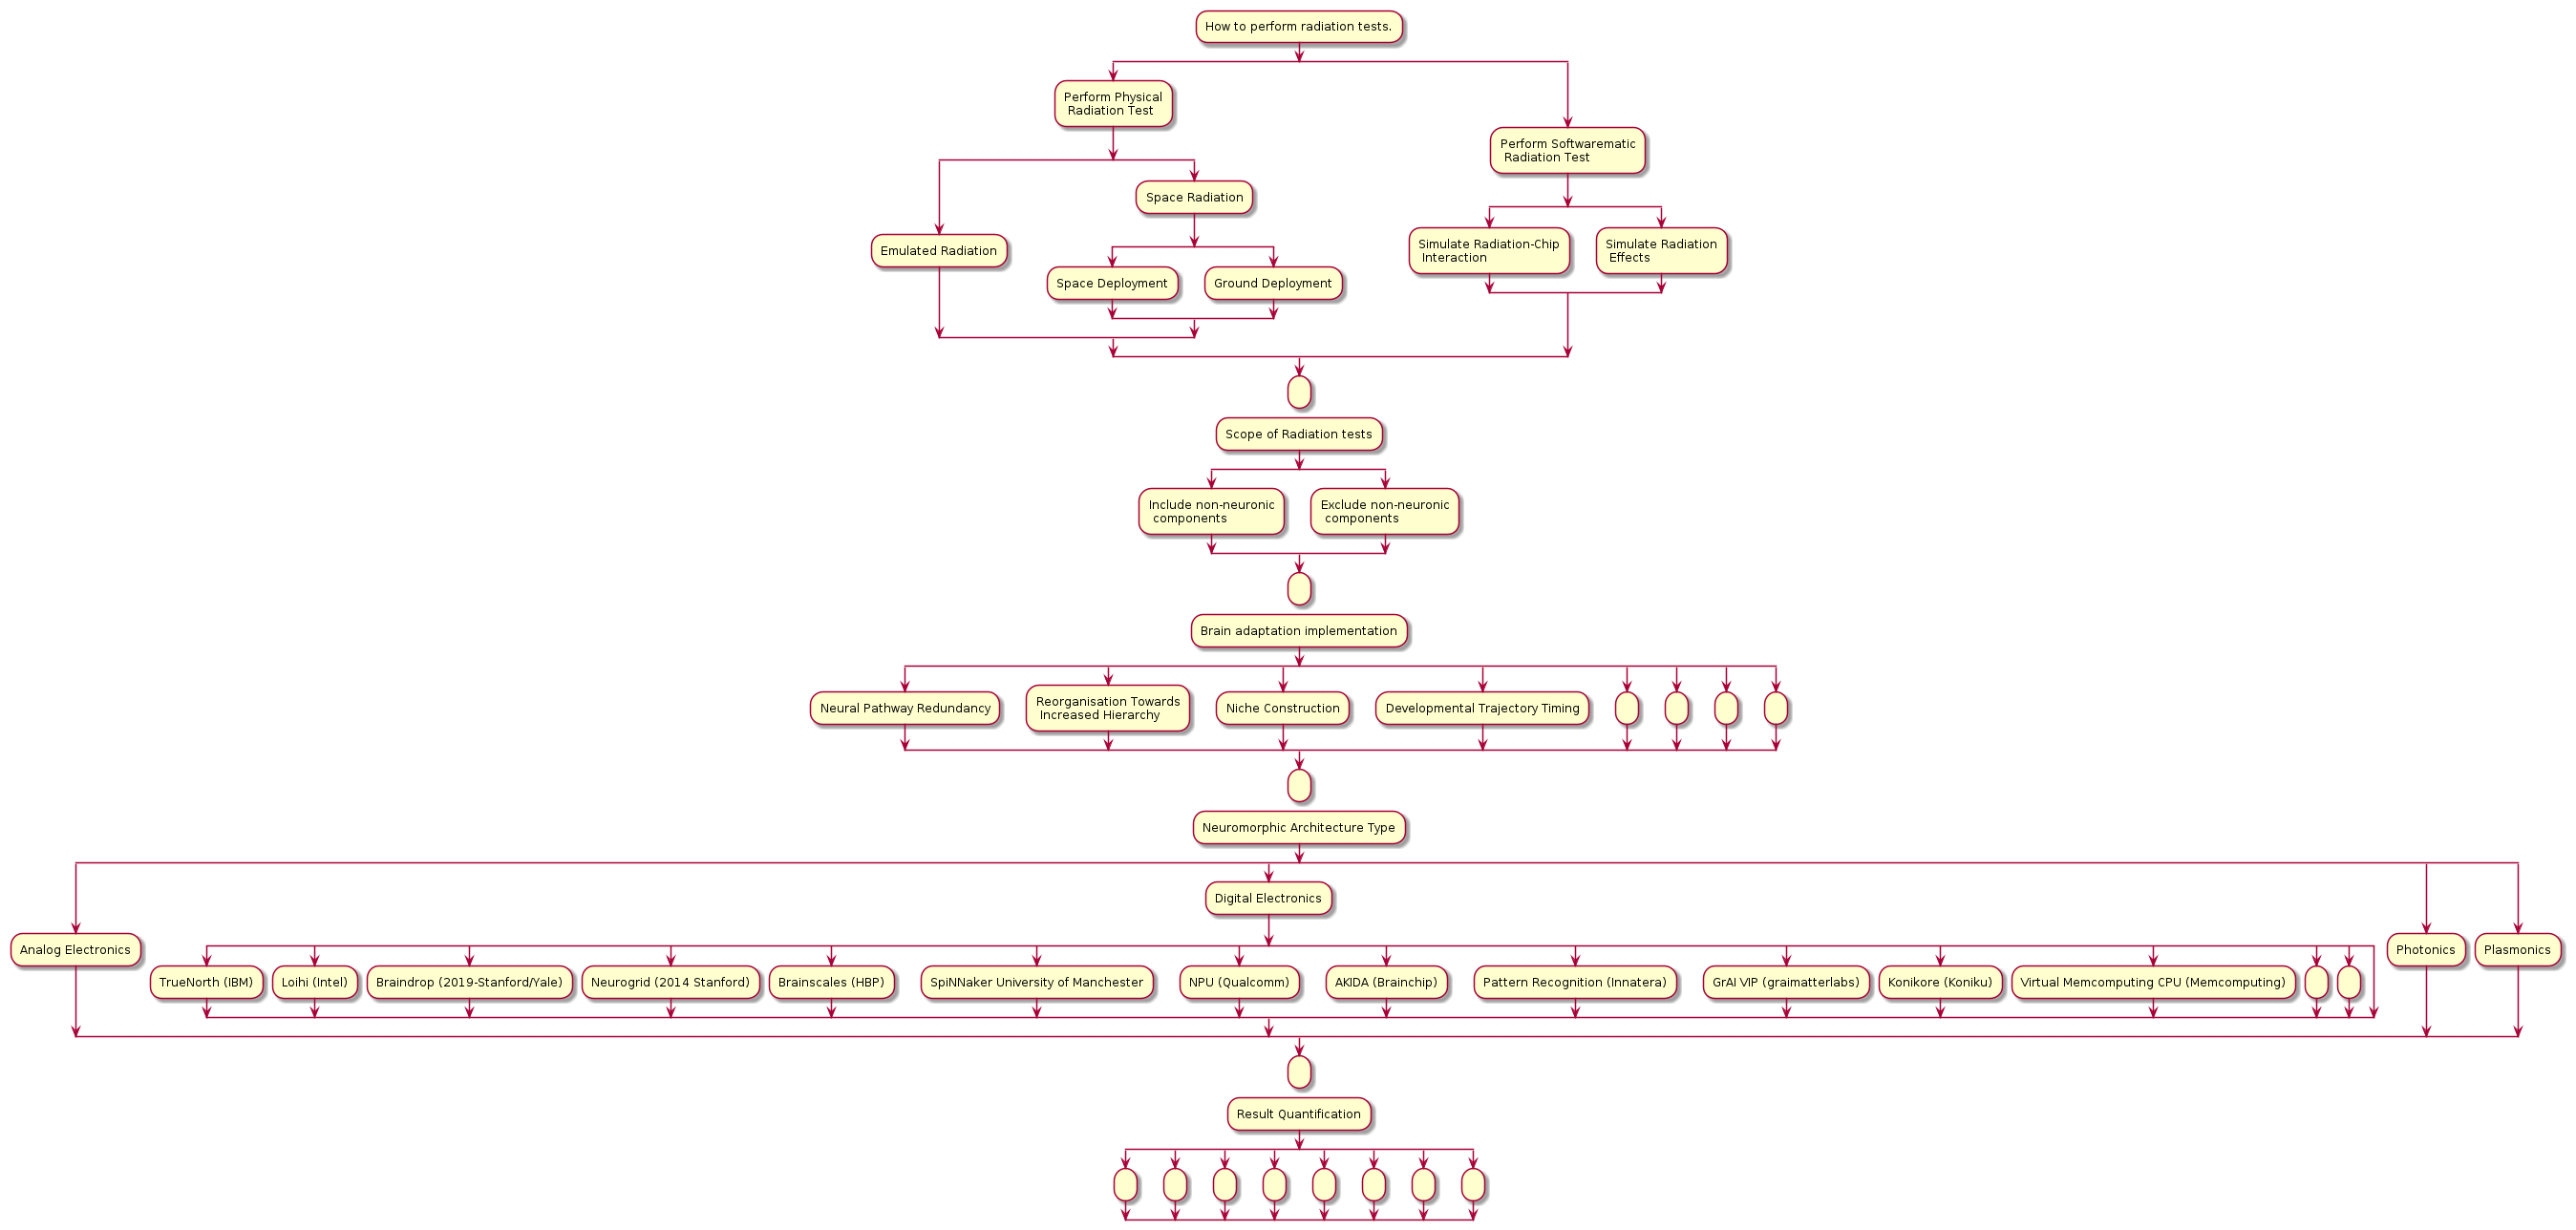
\includegraphics[width=0.6\linewidth]{latex/Images/dot.png}
    \caption{A functional flow diagram with the high-level functions of the system that is to be designed.}
    \label{fig:baseline_dot}
\end{figure}

\section{Pruning}\label{sec:baseline_pruning}
With the design option tree generated, it can be pruned of options that are considered infeasible. This is done using the knowledge base that was generated in the literature study and using the requirements identified in \cref{chap:baseline_requirements_discovery_tree}.  The pruning process will be performed from top to bottom, which matches from high- to low hierarchical design choices.
\subsection{Tested Functionality}\label{subsec:tested_functionality}
At the time of writing, no specific function that is used for testing, can be eliminated.
\subsection{How To Perform Radiation Tests}\label{subsec:baseline_how_to_perform_radiation_tests}
\begin{enumerate}
    \item Starting with key requirement: \textbf{STKH-SPACEBRAINS-01} and \textbf{STKH-ICONS-01}, it is possible to eliminate the physical radiation test design option(along with its children), before the ICONS deadline of April 15th, 2022. Given the full scope of the thesis, and the \textbf{TEST-03} requirement which implies a test deadline before September 2022, a physical radiation test is still considered feasible before that time. Hence, instead of a complete termination (red), it is turned orange.
    \item Continuing with the \textbf{STKH-SPACEBRAINS-01} requirement, it is considered infeasible to do a full simulation of radiation effects on the hardware components, before the ICONS deadline of April 15th, 2022. Hence, also this option will be coloured orange. Most neuromorphic chips in the \acrshort{dot} are proprietary, with many of the chip designs not being publically available. Since that makes it difficult to determine what the radiation effects will be on the hardware components of the chip, and how those effects, such as single-event upsets, would propagate towards influencing neurons and/or synapses. Therefore, this option is not considered feasible before April 15th 2022. It may be possible to contact manufacturers to ask how the radiation influences the neuronal- and synaptic properties. If such research is performed, it may be applied to simulate the neuromorphic hardware-radiation interaction softwarematically with sufficient accuracy to produce meaningful results.
\end{enumerate}   
\subsection{Scope Of Radiation Tests}\label{subsec:baseline_scope_of_radiation_tests}
\begin{enumerate}
    \item For the same as the last enumerated point of \cref{subsec:baseline_how_to_perform_radiation_tests}, including the non-neuromorphic components is not considered feasible for before the ICONS deadline of April 15th, 2022. Hence, this element is also coloured orange.
\end{enumerate}

\subsection{Brain Adaptation Implementation}\label{subsec:baseline_brain_adaptation_implementation}
At the time of writing, no brain adaptation mechanisms can be eliminated.

\subsection{Neuroplasticity Mechanism}\label{subsec:baseline_neuroplasticity_mechanism}
At the time of writing, no neuroplasticitiy mechanisms can be eliminated.

\subsection{Neuromorphic Architecture}\label{subsec:baseline_neuromorphic_architecture}
\begin{enumerate}
    \item Some neuromorphic architectures can be eliminated based on logistical reasons. Currently, the only direct access within this thesis project is to the Loihi. Furthermore, it may be expected that access to Pattern Recognition Chip by Innaterra may be realised after the ICONS deadline. Similarly, the Spinnaker device may become available later-on in the project. An economic feasibility assessment needs to be made on whether they should be used in physical radiation testing or not.
    \item Some of the neuromorphic chip manufacturers have been contacted in the past, these contacts may allow for access to their respective chips for physical radation testing, if the intermediate results at ICONS are promising. Hence, they are kept orange.
\end{enumerate}

\subsection{Result Quantification}\label{subsec:baseline_result_quantification}
\begin{enumerate}
    \item Since physical radiation testing is not deemed possible, and since the hardware diagrams of the respective neuromorphic architectures are not available, it is not deemed feasible to include a radiation effect analysis before ICONS. Therefore, this option is turned orange.
\end{enumerate}

\subsection{Pruned Design Option Tree}\label{subsec:baseline_pruned_dot}
\begin{figure}[H]
    \centering
    %\includegraphics[width=0.6\linewidth]{Images/Diagrams/trivial_gantt.png}
    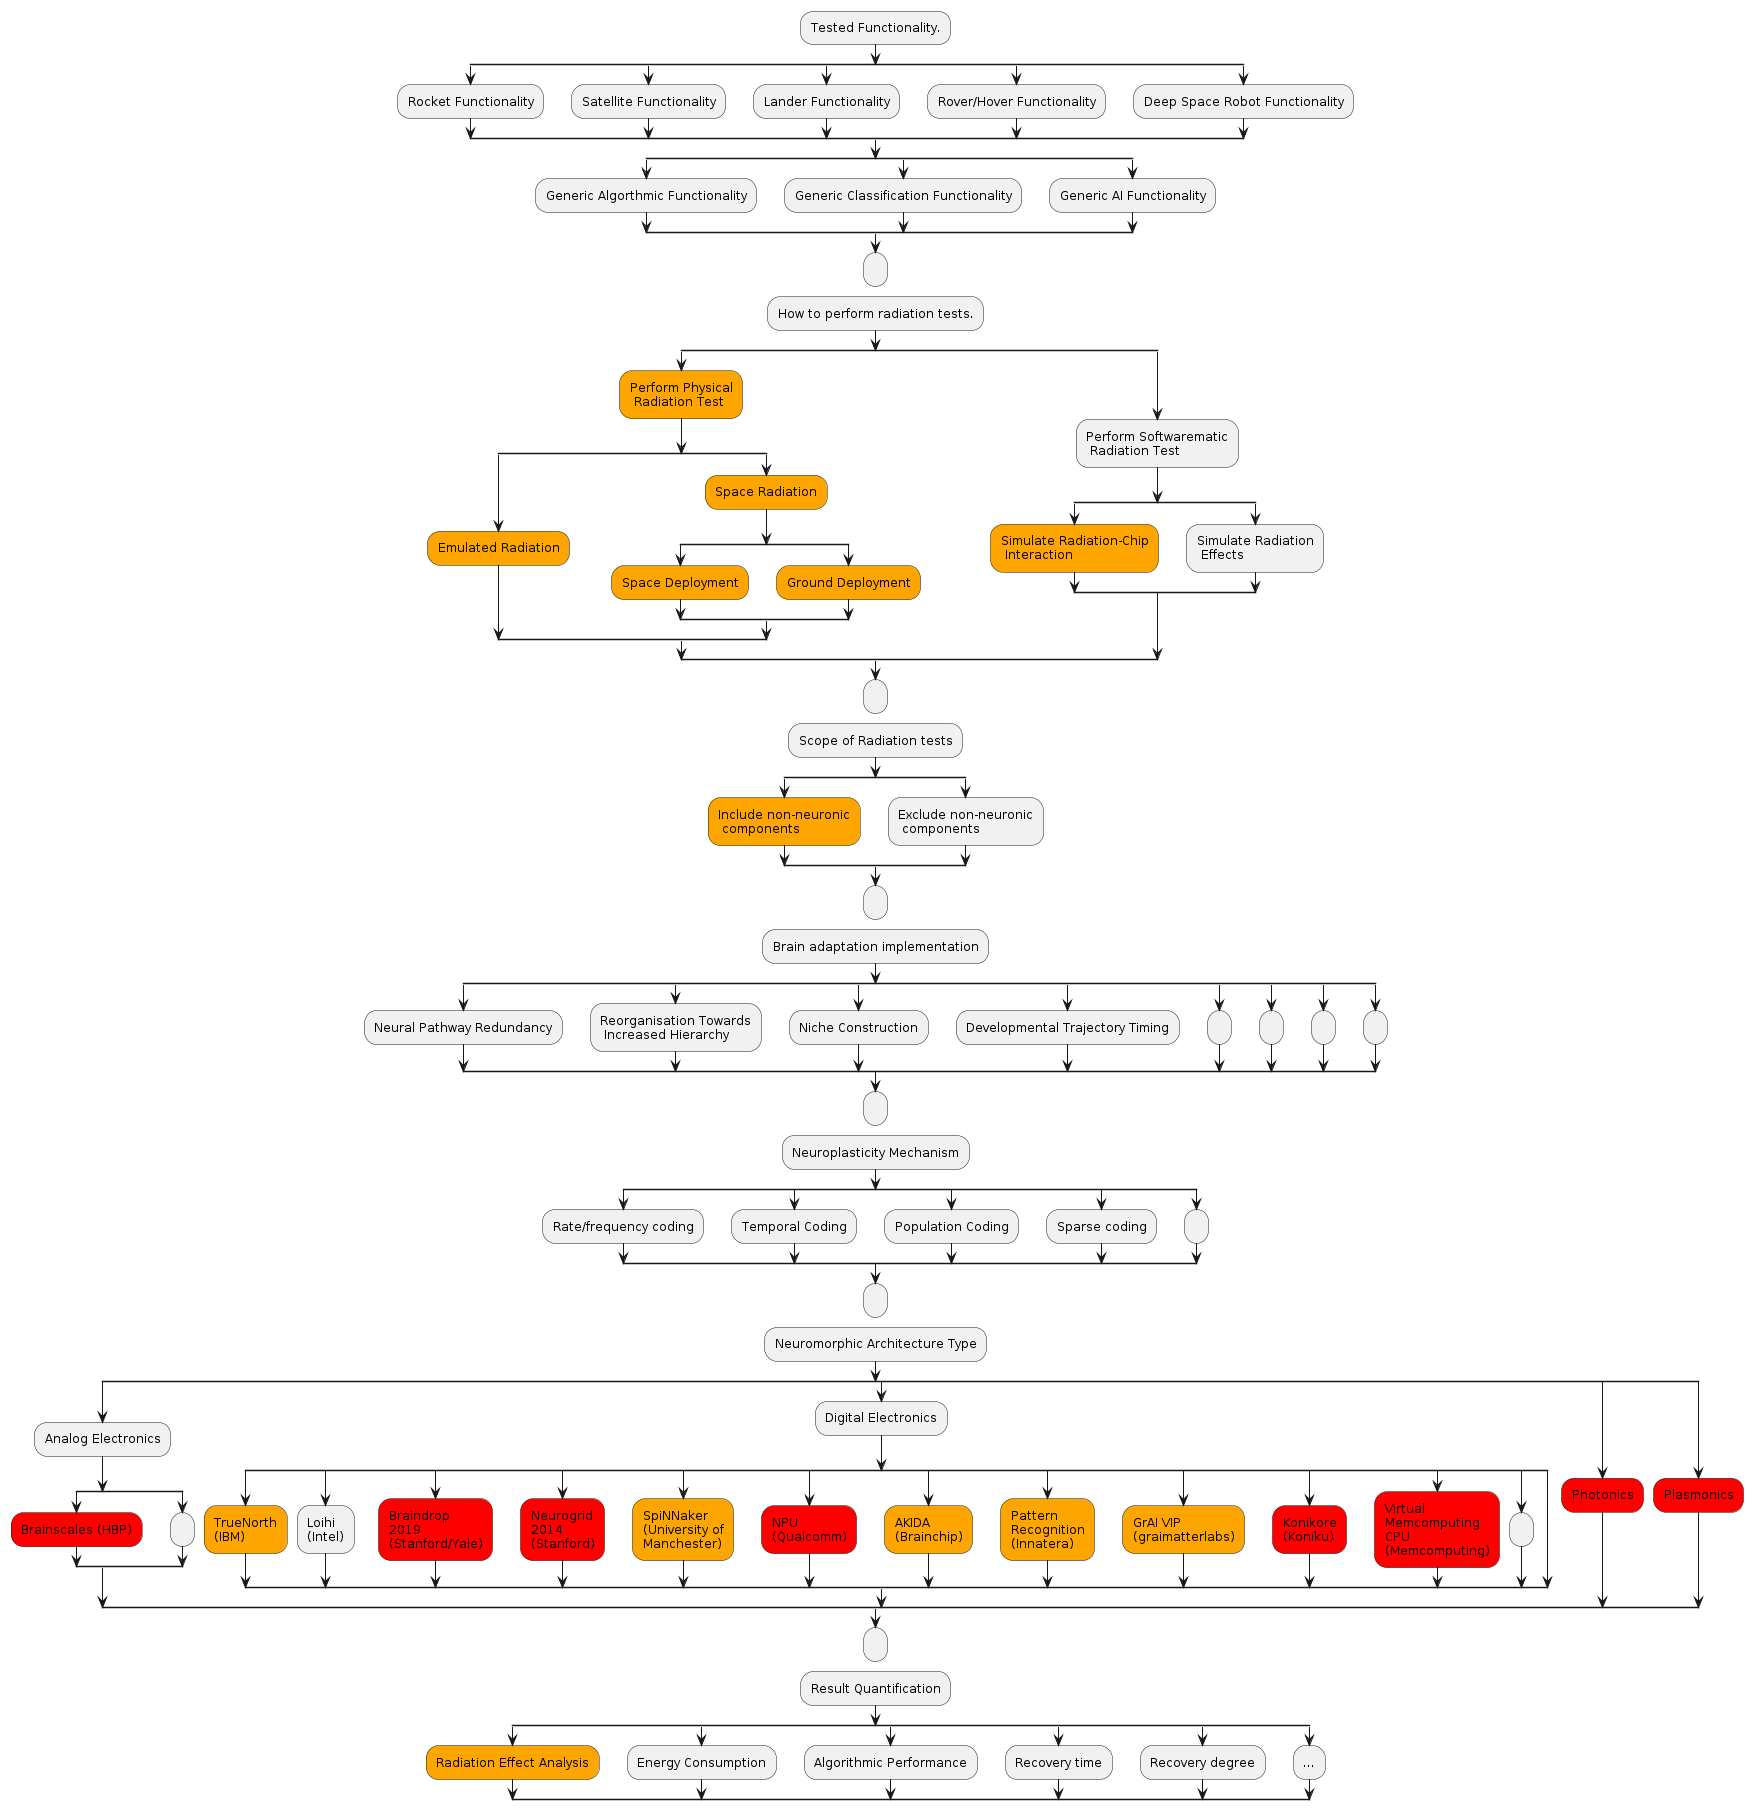
\includegraphics[width=0.6\linewidth]{code/src/Static_diagrams/dot_pruned.png}
    \caption{A functional flow diagram with the high-level functions of the system that is to be designed.}
    \label{fig:baseline_dot}
\end{figure}


\section{Preliminary Design Option Selection}\label{sec:baseline_preliminary_design_option_selection}
With some design options eliminated, an analysis can be performed to see whether some design options are considered to be more feasible than others. This analysis is started by taking the \textbf{STKH-SPACEBRAINS-01} requirement into account, which implies results need to be produced by April 15th. This allows for expressing some design option preferences as listed in \cref{subsec:baseline_tested_functionality_preference} to \cref{subsec:baseline_result_quantification_preference}. Taking the full scope of the thesis project into account allows identification of design options that seem most feasible for a follow-up with physical radiation testing.

\subsection{Tested Functionality Preference}\cref{subsec:baseline_tested_functionality_preference}
For performing a \textit{generic algorithmic functionality} for the following two reasons:
\begin{enumerate}
    \item No additional dependencies such as datasets, panda packages, tensorflow etc. is required. This lowers the probability of allocating time on work that does not directly support the objective of this thesis project.
    \item No preprocessing work, such as loading and/or cropping images etc.,  is required. This increases the amount of time that can be allocated to implementing the brain adaptation and testing its functionality.
    \item Graph algorithms are typically used in space applications \cite{todo}.%, an example is the MDS approximation in communication satellites.
    \item Thorough testing can quickly be set up for graph algorithms.
\end{enumerate}
 
\subsection{How To Perform Radiation Tests Preference}\cref{subsec:baseline_how_to_perform_radiation_tests_preference}
Using softwarematic radiation tests that simulate radiation effects.

\subsection{Scope of Radiation Tests Preference}\cref{subsec:baseline_scope_of_radiation_tests_preference}
Excluding non-neural components from radiation effects allows for a complete focus using the expected radiation effects on the neural and synaptic properties, without having to model additional radiation interactions with (other) hardware elements. This increases the feasibility of producing results by April 15th.

\subsection{Brain Adaptation Implementation Preference}\cref{subsec:baseline_brain_adaptation_implementation_preference}
No preference in brain adaptation implementations is expressed at the time of writing.

\subsection{Neuroplasticity Mechanism Preference}\cref{subsec:baseline_neuroplasticity_mechanism_preference}
No preference in neuroplasticity mechanisms is expressed at the time of writing.

\subsection{Neuromorphic Architecture Type Preference}\cref{subsec:baseline_neuromorphic_architecture_preference}
Based on availability and previous experience, a preference is expressed for the Loihi platform for the softwarematic simulation. Insights from this simulation will be used to determine the best way forward towards hardware simulations. Since the Innatera chips are expected to be available for testing in the second quarter of 2022, combined with there relatively low cost, this option is mentioned as a possible suitable candidate for physical radiation testing. The Spinnaker boards appear to have a higher unit cost.

\subsection{Result Quantification Preference}\cref{subsec:baseline_result_quantification_preference}
Based on the vicinity of the ICONS deadline of April 15th, 2022, a preference is expressed for measuring the softwarematic results in terms of algorithmic performance. This is because it forms the most direct measurement that can be used to determine whether the principle of brain adaptation is indeed able to increase the radiation robustness of neuromorphic space hardware.

\subsection{Preliminary Design Option Tree}\label{subsec:preliminary_design_option_tree}
The preferences expressed in \cref{sec:baseline_preliminary_design_option_selection} are coloured green in the preliminary design option tree visualised in \cref{fig:baseline_preliminary_dot}.

\begin{figure}[H]
    \centering
    %\includegraphics[width=0.6\linewidth]{Images/Diagrams/trivial_gantt.png}
    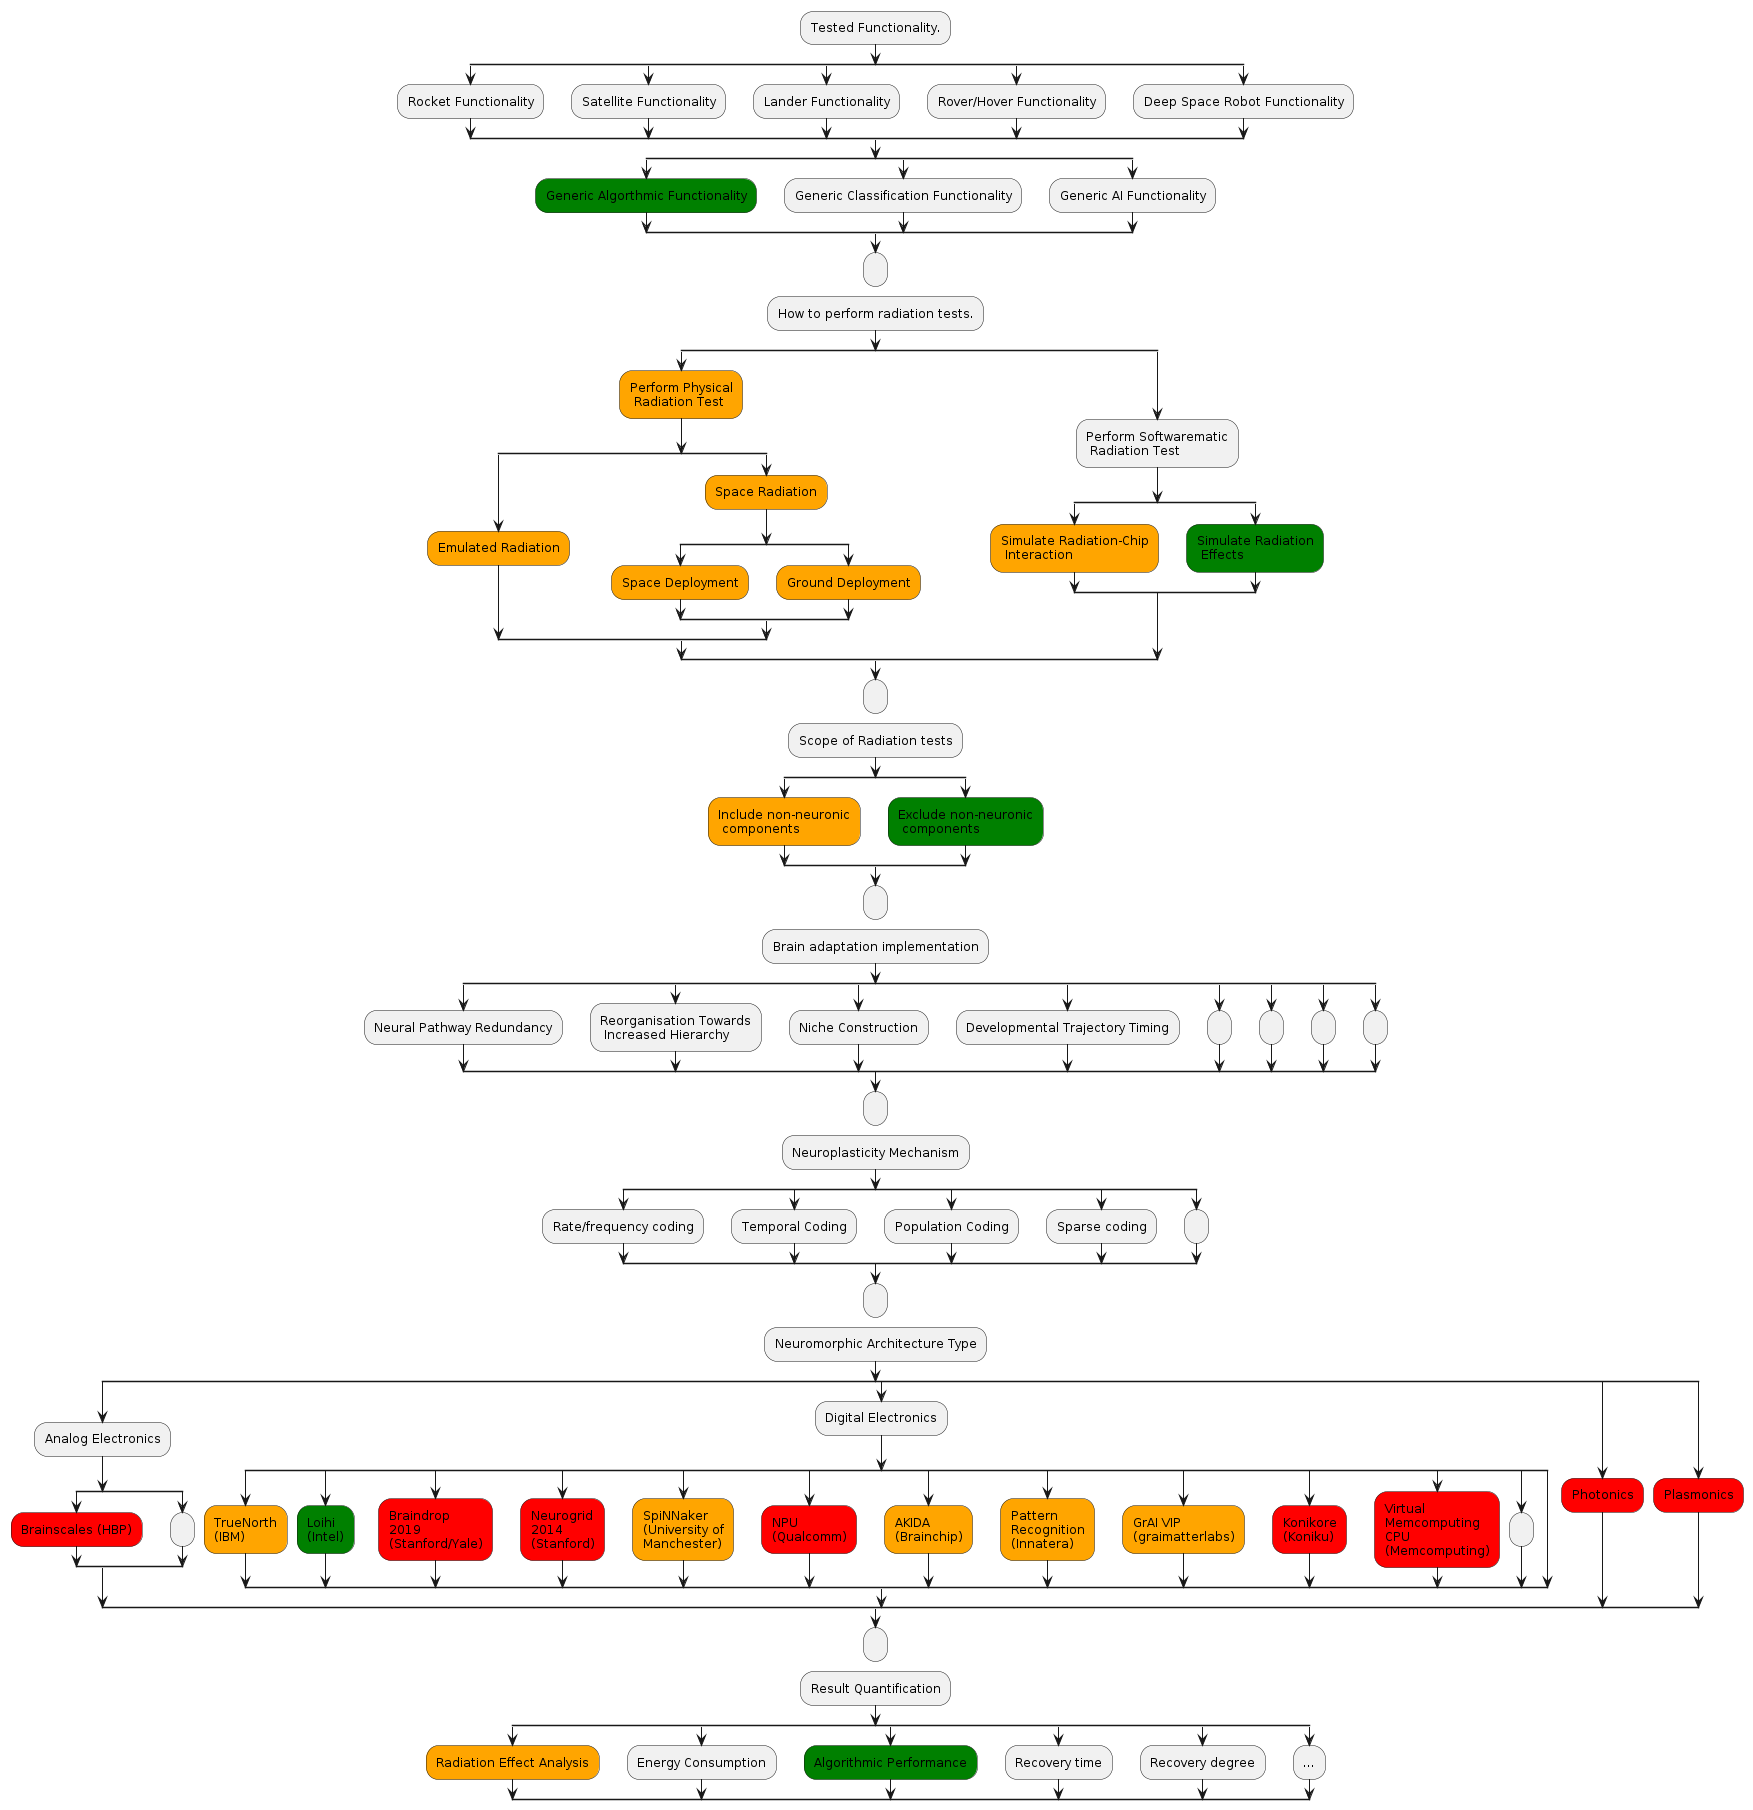
\includegraphics[width=0.6\linewidth]{latex/Images/Diagrams/Static_diagrams/dot_preliminary.png}
    \caption{todo}
    \label{fig:baseline_preliminary_dot}
\end{figure}

\section{Proposed Design options}\label{subsec:baseline_proposed_design options.}
To summarise, a distinction between project phases. First a softwarematic test is performed and the results are reported to the ICONS by  April 15th 2022. Next, a hardwarematic test is proposed that builds upon the knowledge gained in the softwarematic tests. For the first phase, the following options are proposed to be executed during the midterm: A graph algorithm is proposed to be ran, where the radiation effects on the neuromorphic architecture are simulated as changes in the the neural and synaptic properties of the spiking neural networks. For this first softwarematic test, the radiation effects on non-neural/traditional hardware components (such as a memory bus, \acrshort{cpu} etc.) of the neuromorphic architecture are ignored. The Loihi platform will be used for the simulation development and radiation tests. The test results will be interpreted in terms of performance of the graph algorithm. The most feasible brain-adaptation method and neuroplasticitiy mechanism will be determined using hands-on experimentation.
% TODO: change generic alg to graph alg
For the second tests, a physical radiation test is proposed. For this test, the Innatera chips are currently considered as the most feasible option. Based on the results of the softwarematic testing, a decision can be made to inlcude the traditional hardware components of the respective chips. An alternative option could be to apply extra shielding to those components, whilst saving mass on the non-shielded components though the use of brain adaptation inspired implementations.

\chapter{Contingency Management}\label{chap:baseline_contingency_management}
\chapter{Market Analysis}\label{chap:baseline_market_analysis}
\chapter{Sustainable Development Management}\label{chap:baseline_sustainable_development_management}
\chapter{Reporting and Quality Control}\label{chap:baseline_reporting_and_quality_control}
The following quality control compliance checklist can currently be generated for this project plan:

\begin{itemize}
	\item Language Tools Grammar check applied:\greencheck
	\item Language Tools Spelling check applied:\greencheck
	\item CI is ran on code base used in generating this Project Plan:\xmark
	\begin{itemize}
		\item Python Black Formatting Compliance:\xmark
		\item ShellCheck Compliance:\xmark
		\item Latex Prettier Formatting Compliance:\xmark
		\item Python Unit Test Passing: 2 failed, 7 passed [tests]
		\item Python Test Coverage \%:\xmark [\%]
		\item Shell Unit Test Passing:\xmark [tests]
		\item Shell Unit Test Coverage \%:\xmark [\%]
	\end{itemize}
	\item Manual Quality check:
	\begin{enumerate}
		\item Citations still have to be compiled correctly.
		\item Reproduction instructions in Appendix A should be updated.
		\item Word wrap should be applied to .uml appendices.
	\end{enumerate}
\end{itemize}
\chapter{Conclusion}\label{chap:baseline_conclusion}
\fi

%% Use letters for the chapter numbers of the appendices.
\appendix

%\input{appendix-a}

%\bibliography{report}

\newpage
%\appendix
%% Uncomment the following line when using the natbib package
\bibliography{zotero.bib}
%\bibliography{latex/zotero.bib}

%% Uncomment the following line when using the biblatex package
%\printbibliography



\newpage
% Example glossary text:
%Example glossary text: The \Gls{latex} typesetting markup language is specially suitable for documents that include \gls{maths}. \Glspl{formula} are rendered properly an easily once one gets used to the commands.
\printglossary[type=\acronymtype]

\printglossary
\printnomenclature

% Example list of accronyms:
%Given a set of numbers, there are elementary methods to compute its \acrlong{gcd}, which is abbreviated \acrshort{gcd}. This process is similar to that used for the \acrfull{lcm}. Test.


\glsaddall

\newpage
% print acronyms section
%\printglossary[type=\acronymtype,title=Acronyms]
%\printnoidxglossary[type=\acronymtype,title=Acronyms]
% print glossary section
%\printglossary[title=Glossary]
%\printnoidxglossary[title=Glossary]
% print nomenclature
%\newpage
%% Nomenclature is a list of mathematical symbols and their description.
% Source: https://www.overleaf.com/learn/latex/Nomenclatures
%\usepackage[intoc]{nomencl}
%\makenomenclature

% Within document
\mbox{}

\nomenclature{$c$}{Speed of light in a vacuum inertial frame}
\nomenclature{$h$}{Planck constant}

%\newpage
\begin{appendices}
\IfFileExists{latex/report.tex}{\section{Appendix}\label{app:1}
This is a manual appendix. \newpage
}{\section{Appendix}\label{app:1}
This is a manual appendix.} \newpage
\ifhidesourcecode{}\else{\IfFileExists{latex/report.tex}{\section{Appendix Plot\_to\_tex.py}\label{app:3}
\IfFileExists{latex/project6/../../code/project6/src/Plot_to_tex.py}{
\pythonexternal{latex/project6/../../code/project6/src/Plot_to_tex.py}
}{
\pythonexternal{../../code/project6/src/Plot_to_tex.py}
}
 \newpage
\section{Appendix plantuml\_generate.py}\label{app:12}
%TESTCOMMENT
\IfFileExists{latex/../src/export_data/plantuml_generate.py}{
\pythonexternal{latex/../src/export_data/plantuml_generate.py}
}{
\pythonexternal{latex/../src/export_data/plantuml_generate.py}
}
%TESTCOMMENTCLOSING
 \newpage
\section{Appendix Plot\_to\_tex.py}\label{app:6}
%TESTCOMMENT
\IfFileExists{latex/../src/export_data/Plot_to_tex.py}{
\pythonexternal{latex/../src/export_data/Plot_to_tex.py}
}{
\pythonexternal{latex/../src/export_data/Plot_to_tex.py}
}
%TESTCOMMENTCLOSING
 \newpage
\section{Appendix Subgantt.py}\label{app:2}
\IfFileExists{latex/../../code/project6/src/Subgantt.py}{
\pythonexternal{latex/../../code/project6/src/Subgantt.py}
}{
\pythonexternal{../../code/project6/src/Subgantt.py}
}
 \newpage
\section{Appendix Compile\_gantt\_locally.py}\label{app:1}
\IfFileExists{latex/project6/../../code/project6/src/Compile_gantt_locally.py}{
\pythonexternal{latex/project6/../../code/project6/src/Compile_gantt_locally.py}
}{
\pythonexternal{../../code/project6/src/Compile_gantt_locally.py}
}
 \newpage
\section{Appendix Compile\_latex.py}\label{app:4}
\IfFileExists{latex/../../code/project6/src/Compile_latex.py}{
\pythonexternal{latex/../../code/project6/src/Compile_latex.py}
}{
\pythonexternal{../../code/project6/src/Compile_latex.py}
}
 \newpage
\section{Appendix plantuml\_get\_package.py}\label{app:9}
%TESTCOMMENT
\IfFileExists{latex/../src/export_data/plantuml_get_package.py}{
\pythonexternal{latex/../src/export_data/plantuml_get_package.py}
}{
\pythonexternal{latex/../src/export_data/plantuml_get_package.py}
}
%TESTCOMMENTCLOSING
 \newpage
\section{Appendix Plot\_to\_tex.py}\label{app:15}
%TESTCOMMENT
\IfFileExists{latex/project8/../../code/project8/src/Plot_to_tex.py}{
\pythonexternal{latex/project8/../../code/project8/src/Plot_to_tex.py}
}{
\pythonexternal{../../code/project8/src/Plot_to_tex.py}
}
%TESTCOMMENTCLOSING
 \newpage
\section{Appendix plantuml\_compile.py}\label{app:14}
%TESTCOMMENT
\IfFileExists{latex/../src/export_data/plantuml_compile.py}{
\pythonexternal{latex/../src/export_data/plantuml_compile.py}
}{
\pythonexternal{latex/../src/export_data/plantuml_compile.py}
}
%TESTCOMMENTCLOSING
 \newpage
\section{Appendix helper\_dir\_file\_edit.py}\label{app:16}
%TESTCOMMENT
\IfFileExists{latex/../src/export_data/helper_dir_file_edit.py}{
\pythonexternal{latex/../src/export_data/helper_dir_file_edit.py}
}{
\pythonexternal{latex/../src/export_data/helper_dir_file_edit.py}
}
%TESTCOMMENTCLOSING
 \newpage
\section{Appendix Work\_flow\_diagram.py}\label{app:10}
\IfFileExists{latex/project6/../../code/project6/src/Work_flow_diagram.py}{
\pythonexternal{latex/project6/../../code/project6/src/Work_flow_diagram.py}
}{
\pythonexternal{../../code/project6/src/Work_flow_diagram.py}
}
 \newpage
\section{Appendix neumann.py}\label{app:0}
%TESTCOMMENT
\IfFileExists{latex/../src/neumann.py}{
\pythonexternal{latex/../src/neumann.py}
}{
\pythonexternal{latex/../src/neumann.py}
}
%TESTCOMMENTCLOSING
 \newpage
\section{Appendix Deliverable.py}\label{app:5}
\IfFileExists{latex/project6/../../code/project6/src/Deliverable.py}{
\pythonexternal{latex/project6/../../code/project6/src/Deliverable.py}
}{
\pythonexternal{../../code/project6/src/Deliverable.py}
}
 \newpage
\section{Appendix Work\_breakdown\_structure.py}\label{app:13}
\IfFileExists{latex/project6/../../code/project6/src/Work_breakdown_structure.py}{
\pythonexternal{latex/project6/../../code/project6/src/Work_breakdown_structure.py}
}{
\pythonexternal{../../code/project6/src/Work_breakdown_structure.py}
}
 \newpage
\section{Appendix latex\_export\_code.py}\label{app:11}
%TESTCOMMENT
\IfFileExists{latex/../src/export_data/latex_export_code.py}{
\pythonexternal{latex/../src/export_data/latex_export_code.py}
}{
\pythonexternal{latex/../src/export_data/latex_export_code.py}
}
%TESTCOMMENTCLOSING
 \newpage
\section{Appendix Main.py}\label{app:8}
\IfFileExists{latex/../../code/project6/src/Main.py}{
\pythonexternal{latex/../../code/project6/src/Main.py}
}{
\pythonexternal{../../code/project6/src/Main.py}
}
 \newpage
\section{Appendix plantuml\_to\_tex.py}\label{app:7}
%TESTCOMMENT
\IfFileExists{latex/../src/export_data/plantuml_to_tex.py}{
\pythonexternal{latex/../src/export_data/plantuml_to_tex.py}
}{
\pythonexternal{latex/../src/export_data/plantuml_to_tex.py}
}
%TESTCOMMENTCLOSING
 \newpage
}{\section{Appendix Plot\_to\_tex.py}\label{app:3}
\IfFileExists{latex/project6/../../code/project6/src/Plot_to_tex.py}{
\pythonexternal{latex/project6/../../code/project6/src/Plot_to_tex.py}
}{
\pythonexternal{../../code/project6/src/Plot_to_tex.py}
}
 \newpage
\section{Appendix plantuml\_generate.py}\label{app:12}
%TESTCOMMENT
\IfFileExists{latex/../src/export_data/plantuml_generate.py}{
\pythonexternal{latex/../src/export_data/plantuml_generate.py}
}{
\pythonexternal{latex/../src/export_data/plantuml_generate.py}
}
%TESTCOMMENTCLOSING
 \newpage
\section{Appendix Plot\_to\_tex.py}\label{app:6}
%TESTCOMMENT
\IfFileExists{latex/../src/export_data/Plot_to_tex.py}{
\pythonexternal{latex/../src/export_data/Plot_to_tex.py}
}{
\pythonexternal{latex/../src/export_data/Plot_to_tex.py}
}
%TESTCOMMENTCLOSING
 \newpage
\section{Appendix Subgantt.py}\label{app:2}
\IfFileExists{latex/../../code/project6/src/Subgantt.py}{
\pythonexternal{latex/../../code/project6/src/Subgantt.py}
}{
\pythonexternal{../../code/project6/src/Subgantt.py}
}
 \newpage
\section{Appendix Compile\_gantt\_locally.py}\label{app:1}
\IfFileExists{latex/project6/../../code/project6/src/Compile_gantt_locally.py}{
\pythonexternal{latex/project6/../../code/project6/src/Compile_gantt_locally.py}
}{
\pythonexternal{../../code/project6/src/Compile_gantt_locally.py}
}
 \newpage
\section{Appendix Compile\_latex.py}\label{app:4}
\IfFileExists{latex/../../code/project6/src/Compile_latex.py}{
\pythonexternal{latex/../../code/project6/src/Compile_latex.py}
}{
\pythonexternal{../../code/project6/src/Compile_latex.py}
}
 \newpage
\section{Appendix plantuml\_get\_package.py}\label{app:9}
%TESTCOMMENT
\IfFileExists{latex/../src/export_data/plantuml_get_package.py}{
\pythonexternal{latex/../src/export_data/plantuml_get_package.py}
}{
\pythonexternal{latex/../src/export_data/plantuml_get_package.py}
}
%TESTCOMMENTCLOSING
 \newpage
\section{Appendix Plot\_to\_tex.py}\label{app:15}
%TESTCOMMENT
\IfFileExists{latex/project8/../../code/project8/src/Plot_to_tex.py}{
\pythonexternal{latex/project8/../../code/project8/src/Plot_to_tex.py}
}{
\pythonexternal{../../code/project8/src/Plot_to_tex.py}
}
%TESTCOMMENTCLOSING
 \newpage
\section{Appendix plantuml\_compile.py}\label{app:14}
%TESTCOMMENT
\IfFileExists{latex/../src/export_data/plantuml_compile.py}{
\pythonexternal{latex/../src/export_data/plantuml_compile.py}
}{
\pythonexternal{latex/../src/export_data/plantuml_compile.py}
}
%TESTCOMMENTCLOSING
 \newpage
\section{Appendix helper\_dir\_file\_edit.py}\label{app:16}
%TESTCOMMENT
\IfFileExists{latex/../src/export_data/helper_dir_file_edit.py}{
\pythonexternal{latex/../src/export_data/helper_dir_file_edit.py}
}{
\pythonexternal{latex/../src/export_data/helper_dir_file_edit.py}
}
%TESTCOMMENTCLOSING
 \newpage
\section{Appendix Work\_flow\_diagram.py}\label{app:10}
\IfFileExists{latex/project6/../../code/project6/src/Work_flow_diagram.py}{
\pythonexternal{latex/project6/../../code/project6/src/Work_flow_diagram.py}
}{
\pythonexternal{../../code/project6/src/Work_flow_diagram.py}
}
 \newpage
\section{Appendix neumann.py}\label{app:0}
%TESTCOMMENT
\IfFileExists{latex/../src/neumann.py}{
\pythonexternal{latex/../src/neumann.py}
}{
\pythonexternal{latex/../src/neumann.py}
}
%TESTCOMMENTCLOSING
 \newpage
\section{Appendix Deliverable.py}\label{app:5}
\IfFileExists{latex/project6/../../code/project6/src/Deliverable.py}{
\pythonexternal{latex/project6/../../code/project6/src/Deliverable.py}
}{
\pythonexternal{../../code/project6/src/Deliverable.py}
}
 \newpage
\section{Appendix Work\_breakdown\_structure.py}\label{app:13}
\IfFileExists{latex/project6/../../code/project6/src/Work_breakdown_structure.py}{
\pythonexternal{latex/project6/../../code/project6/src/Work_breakdown_structure.py}
}{
\pythonexternal{../../code/project6/src/Work_breakdown_structure.py}
}
 \newpage
\section{Appendix latex\_export\_code.py}\label{app:11}
%TESTCOMMENT
\IfFileExists{latex/../src/export_data/latex_export_code.py}{
\pythonexternal{latex/../src/export_data/latex_export_code.py}
}{
\pythonexternal{latex/../src/export_data/latex_export_code.py}
}
%TESTCOMMENTCLOSING
 \newpage
\section{Appendix Main.py}\label{app:8}
\IfFileExists{latex/../../code/project6/src/Main.py}{
\pythonexternal{latex/../../code/project6/src/Main.py}
}{
\pythonexternal{../../code/project6/src/Main.py}
}
 \newpage
\section{Appendix plantuml\_to\_tex.py}\label{app:7}
%TESTCOMMENT
\IfFileExists{latex/../src/export_data/plantuml_to_tex.py}{
\pythonexternal{latex/../src/export_data/plantuml_to_tex.py}
}{
\pythonexternal{latex/../src/export_data/plantuml_to_tex.py}
}
%TESTCOMMENTCLOSING
 \newpage
}}\fi\ifhidesourcecode{}\else{\IfFileExists{latex/report.tex}{}{}}\fi\end{appendices}
\end{document}